% !TEX root = ../main.tex

\chapter{Results} \label{ch:results}

%----------------------------------------
% EXPERIMENTS
%----------------------------------------
\section{Experiments}

	The experiments were run using Cessna 172S flight data produced by students at the University of North Dakota during the month of September 2015.  Student flight data is ideal for unstable analysis testing as it contains very noisy data, which provides a diverse array of flying patterns.  A random sample of 100 flights was chosen for the experiments.
        
    First, the application was run against the 100 flights to obtain the automated analysis results.  The same 100 flights were then manually analyzed in order to get human results for the phase identification, which could be compared to the automated results then determine the accuracy of the application.  The test of the 100 flights was also run ten times each with the single-process version and the multi-process version as previously described.  This was done in order to compare and contrast the performance of the separate versions.


%----------------------------------------
% ACCURACY OF PHASE IDENTIFICATION
%----------------------------------------
\section{Accuracy of Phase Identification}

	The manual validation was performed using a combination of tools available on the NGAFID website:  the Cesium flight reanimation tool and the Keyhole Markup Language (KML) generator to visualize the flight path in \textit{Google Earth}~\cite{nolan2014keyhole} (see \Cref{fig:kml_example}).
    
    \begin{figure}
    	\centering
        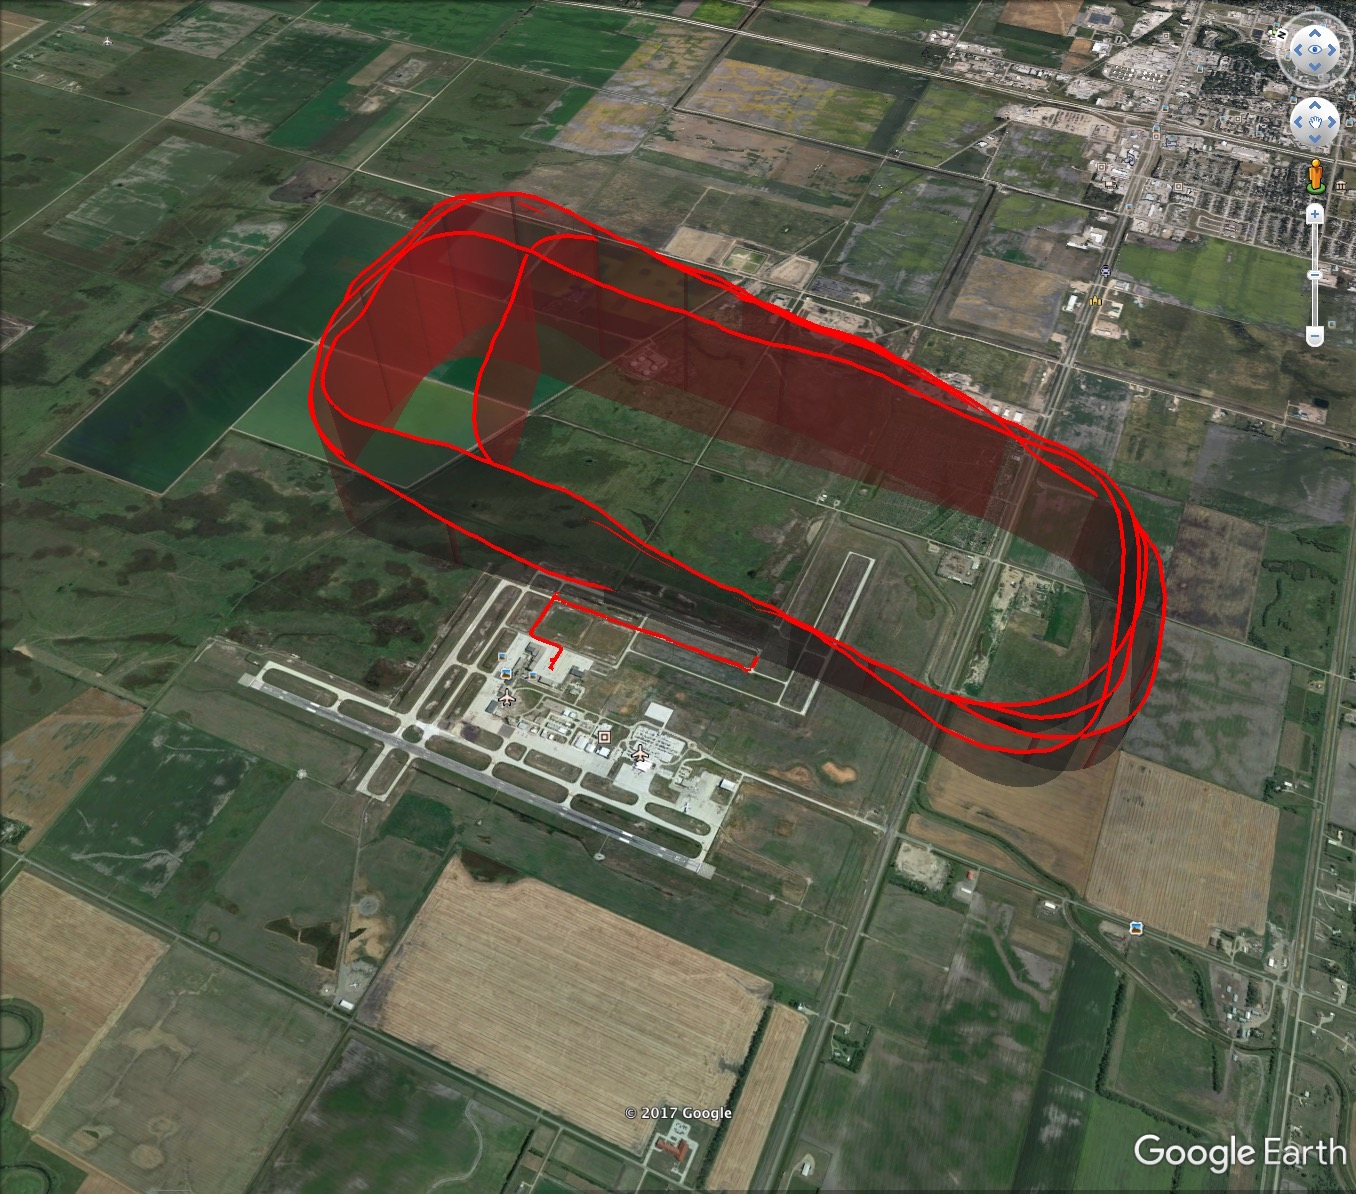
\includegraphics[width=\linewidth]{kml_example}
        \caption{Example of using a KML file to visualize a flight path in \textit{Google Earth}.  This flight visualization is an example of a student flight that has multiple Approach phases.}
        \label{fig:kml_example}
    \end{figure}
    
    
    %----------
    % APPROACH
    %----------
    \subsection{Approach}
    
        The \toolname\ generated a total of 380 approaches for the 100 flights that were tested. As seen in \Cref{fig:kml_example}, student flights typically consist of multiple approaches as this is something that needs to be practiced.  Out of the total; there are 3730 (98.16\%) true positives, five (1.32\%) false positives, and two (0.53\%) false negatives.  These results can also be found in \Cref{fig:validation_results}.
        
        In the context of this application, a true positive is a case where the tool correctly indicates that an approach is occurring during a specified time frame.
        
        A false positive occurs when the tool indicates that an approach is occurring but is not in reality.  Typically, a false positive occurs when the flight data has invalid values for about the first ten rows, which then throws off the beginning of the algorithms.  This happens infrequently, but could be accounted for in a future work by sanitizing the data before analysis.
        
        A false negative is the exact opposite where the tool indicates that an approach is not occurring but it is in reality.  Typically, a false negative occurs when the approached runway's geological data is not contained within the database.  These types of occurrences should stop once the airport and runway databases are expanded with more entries.
        
        The tool misclassified the approached runway 13 times (3.42\%).  A runway is misclassified when the difference between the aircraft and runway headings is greater than $20^\circ$.  This occurs during the runway detection portion of the approach analysis algorithm, and the algorithm either returns a \emph{null} runway or an incorrect runway due to the large heading difference.  Lastly, there was a total of 42 (11.05\%) approaches that were given a \textit{null} runway.  This number overlaps with some of the 13 misclassifications, while the rest are due to a lack of runway information as mentioned previously.

        In this same context, it is difficult to quantify the number of true negatives since these would be cases where the tool correctly indicates that an approach is not occurring.  The difficulty lies in how to define a single occurrence.  Should a single true negative be counted for every second the tool indicates that an approach is not occurring?  If so, then this would create a numerous amount of true negatives and would dilute the percentages of the other statistics, which are more important in this application.

        The validation results demonstrate that the \toolname\ is exceptionally accurate in its ability to appropriately detect and classify most approaches in a flight.

        \begin{figure}
            \centering
            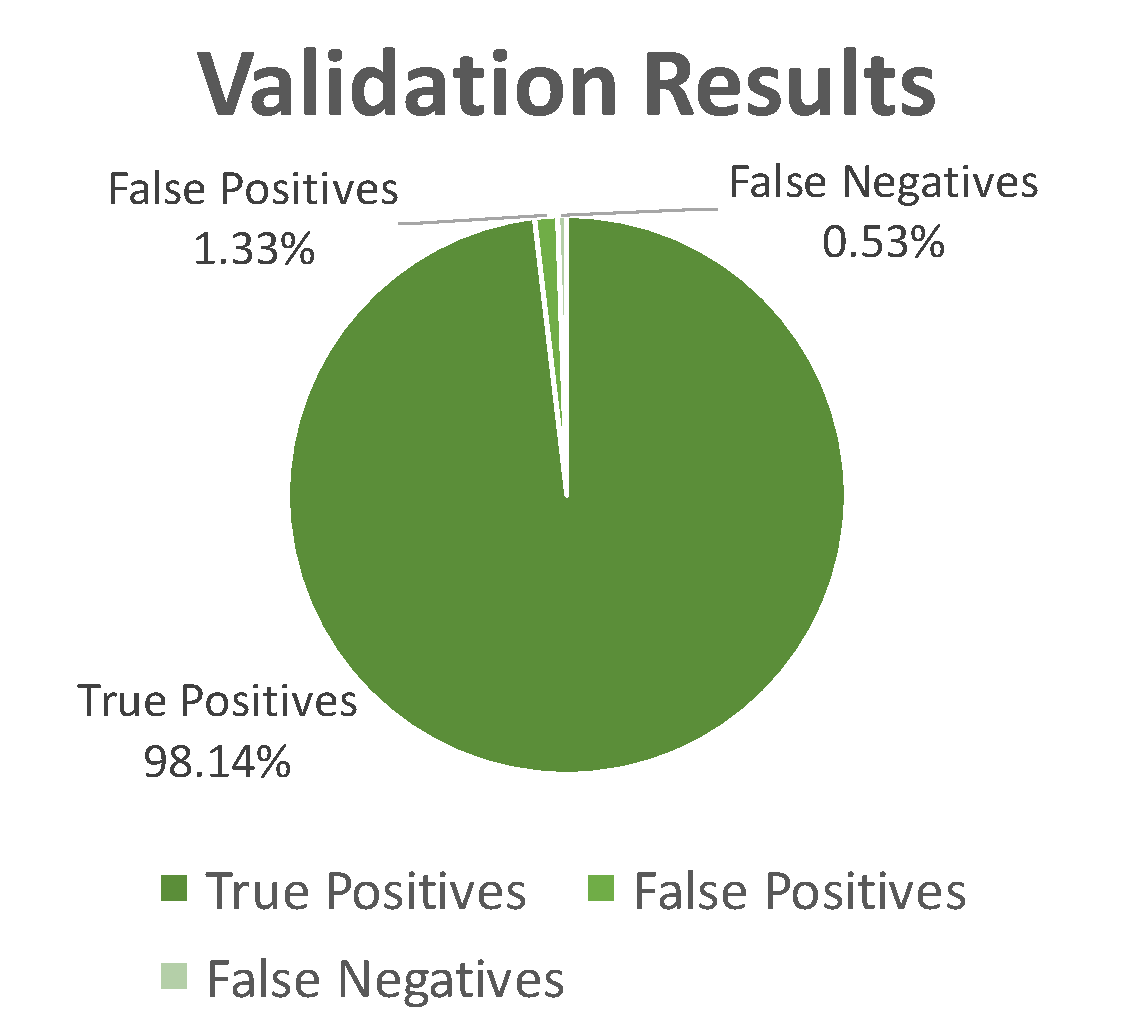
\includegraphics[width=0.85\linewidth]{validation_results}
            \caption{Pie chart showing the manual validation results including true positives, false positives, and false negatives.}
            \label{fig:validation_results}
        \end{figure}
    
    
%----------------------------------------
% QUALITY ANALYSIS RESULTS
%----------------------------------------
\section{Quality Analysis}


	%----------
    % APPROACH
    %----------
    \subsection{Approach}
    
    	The results of the application have provided many possibilities for statistical analysis since numerous statistics can be calculated from the generated approach data.  This can be seen in \Cref{subfig:stableness_results,subfig:unstable_landing_results,subfig:unstable_parameters,subfig:landing_type_results} in which a sample of the possible results were calculated from the experiments of the 100 flights used in this research.  With these various results, trends can be found in the data that has been analyzed.  For example, we can see in \Cref{subfig:stableness_results} that out of the 380 approaches in the sample data, 57.11\% (217) were stable and 42.89\% (163) were unstable.  By drilling down into that data, we can see the frequency for each of the landing types for stable and unstable approaches.  \Cref{subfig:landing_type_results} depicts this more detailed information and shows that full-stop landings occur most frequently for both stable and unstable approaches.  This result is not very surprising for stable approaches; however, it is very undesirable for unstable approaches.  If we look even further into the proportions for unstable approaches alone (\Cref{subfig:unstable_landing_results}), we see that an unstable approach resulted in a go-around only 34.97\% of the time.  This is far lower than the hopeful 100\%, but was expected to be approximately 20\% by our aviation safety experts.  As mentioned previously, this is largely due to pilot misjudgment since all the analyzed flights were piloted by aviation students; meaning they are still learning and are not yet professionals.
    
    When looking at the unstable approaches and the parameters that caused them (\Cref{subfig:unstable_parameters}), additional interesting results can be found.  We found the parameter that was exceeded the most was heading with 91 occurrences.  Heading was not predicted to be the leading cause of unstable approaches, but our safety experts believe the 10$^\circ$ threshold (as defined in \Cref{tab:approach_thresholds}) may be too strict.  Indicated airspeed was the second highest, but was predicted to be the leading cause since it was stated by our aviation safety experts to be a trend for UND's student pilots to be going too fast on final approaches.
    
    \begin{figure}
    	\centering
        \subfloat[Pie chart showing the number of stable approaches compared to the number of unstable approaches.\label{subfig:stableness_results}]{
        	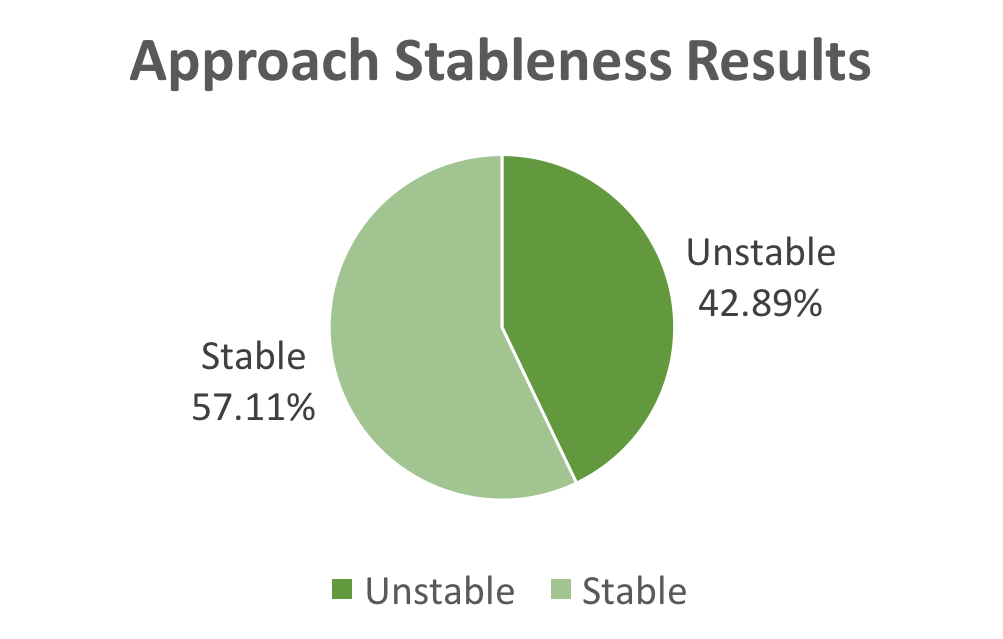
\includegraphics[width=0.45\linewidth]{stableness_results}
        }\hfill%
        \subfloat[Frequency of the occurrences of each landing type for stable and unstable approaches.\label{subfig:landing_type_results}]{
        	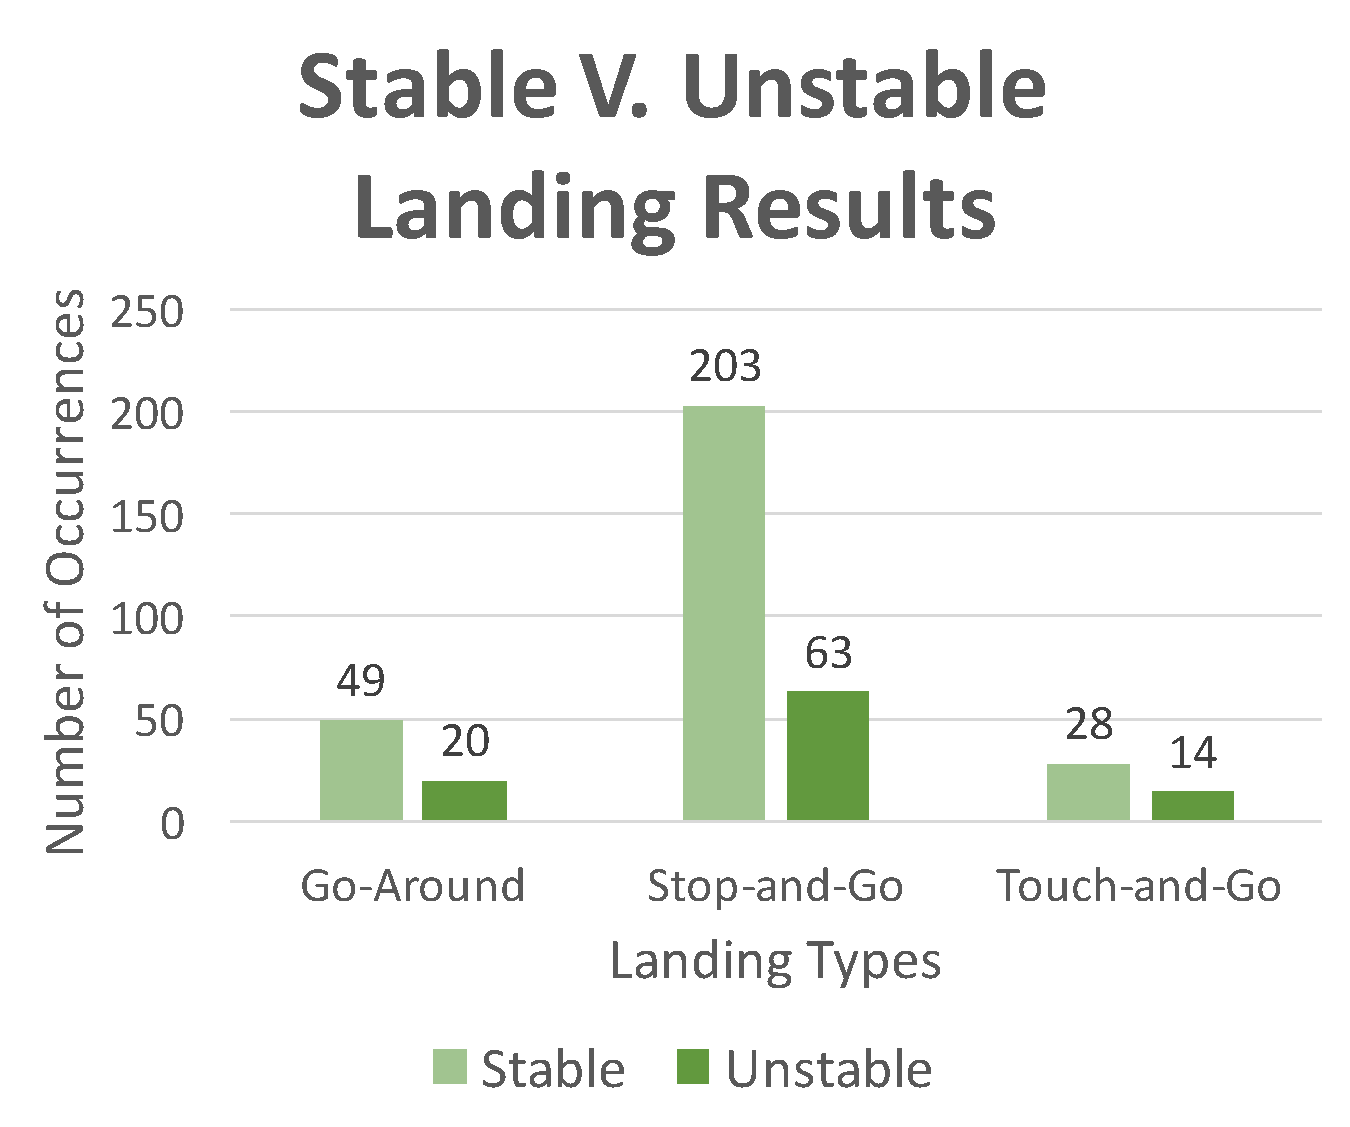
\includegraphics[width=0.45\linewidth]{landing_type_results}
        }%
        
        \subfloat[Pie chart comparing the number of occurrences for each landing type after an unstable approach.\label{subfig:unstable_landing_results}]{
        	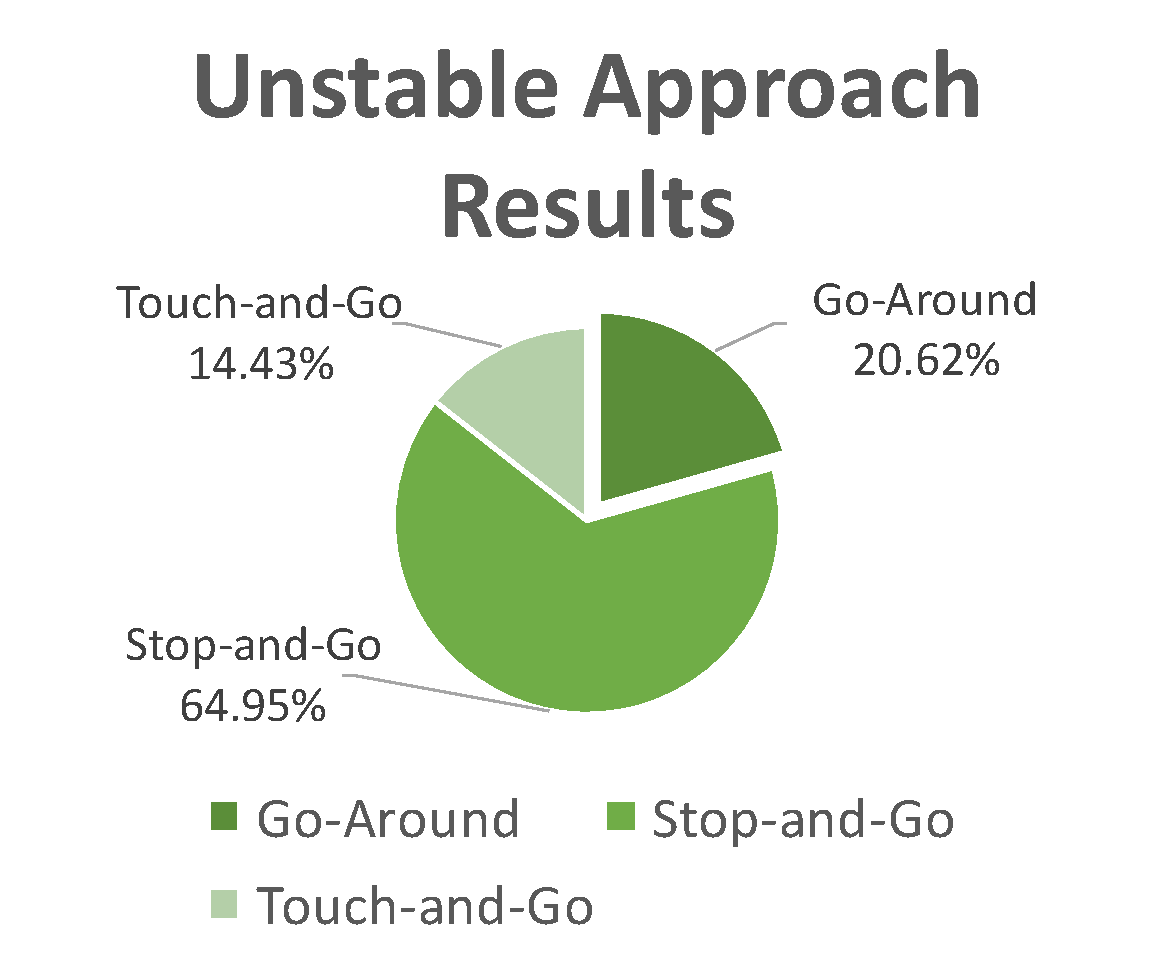
\includegraphics[width=0.45\linewidth]{img/unstable_approach_landing_results}
        }\hfill%
        \subfloat[Frequency of parameters that caused an aircraft to be unstable during an approach.  Note that a single approach can have multiple unstable parameters, which causes the sum of the occurrences to not equal the total number of unstable approaches.\label{subfig:unstable_parameters}]{
        	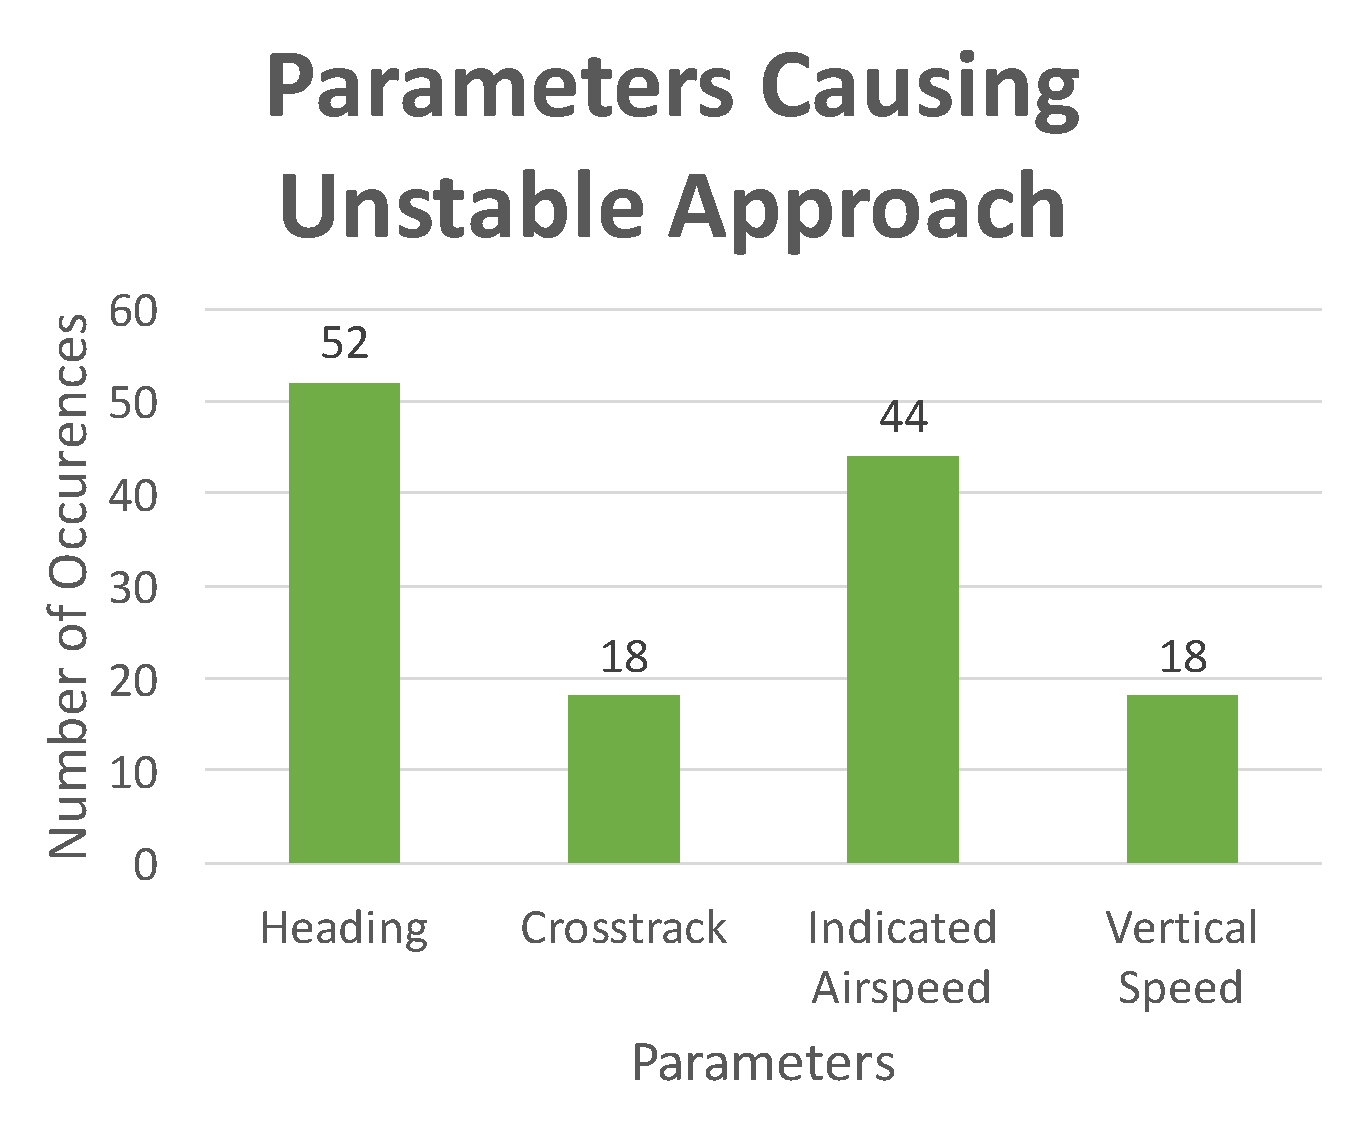
\includegraphics[width=0.45\linewidth]{unstable_parameter_results}
        }%
        \caption{Sample set of the statistics and trends that can be found from the automated analysis results.}
        \label{fig:example_statistics}
    \end{figure}
    
    
    Another interesting set of statistics that can be drawn from the analysis are parameter value frequencies.  Creating histograms of the values for each parameter during all Approach phases can show the values that occur most frequently (highest density).  \Cref{subfig:approach_ias_hist,subfig:approach_vsi_hist,subfig:approach_cross_track_hist,subfig:approach_heading_hist} visualize these histograms and give the corresponding mean and standard deviation values.  These graphs are able to show how well pilots are adhering to the published stabilized approach criteria (see \Cref{tab:approach_thresholds}).  As mentioned previously, the standard deviations will be used in defining the grading metrics and will be discussed in more detail later in this Chapter.
    
    \begin{figure}
    	\centering
        \subfloat[Indicated airspeed.\label{subfig:approach_ias_hist}]{
        	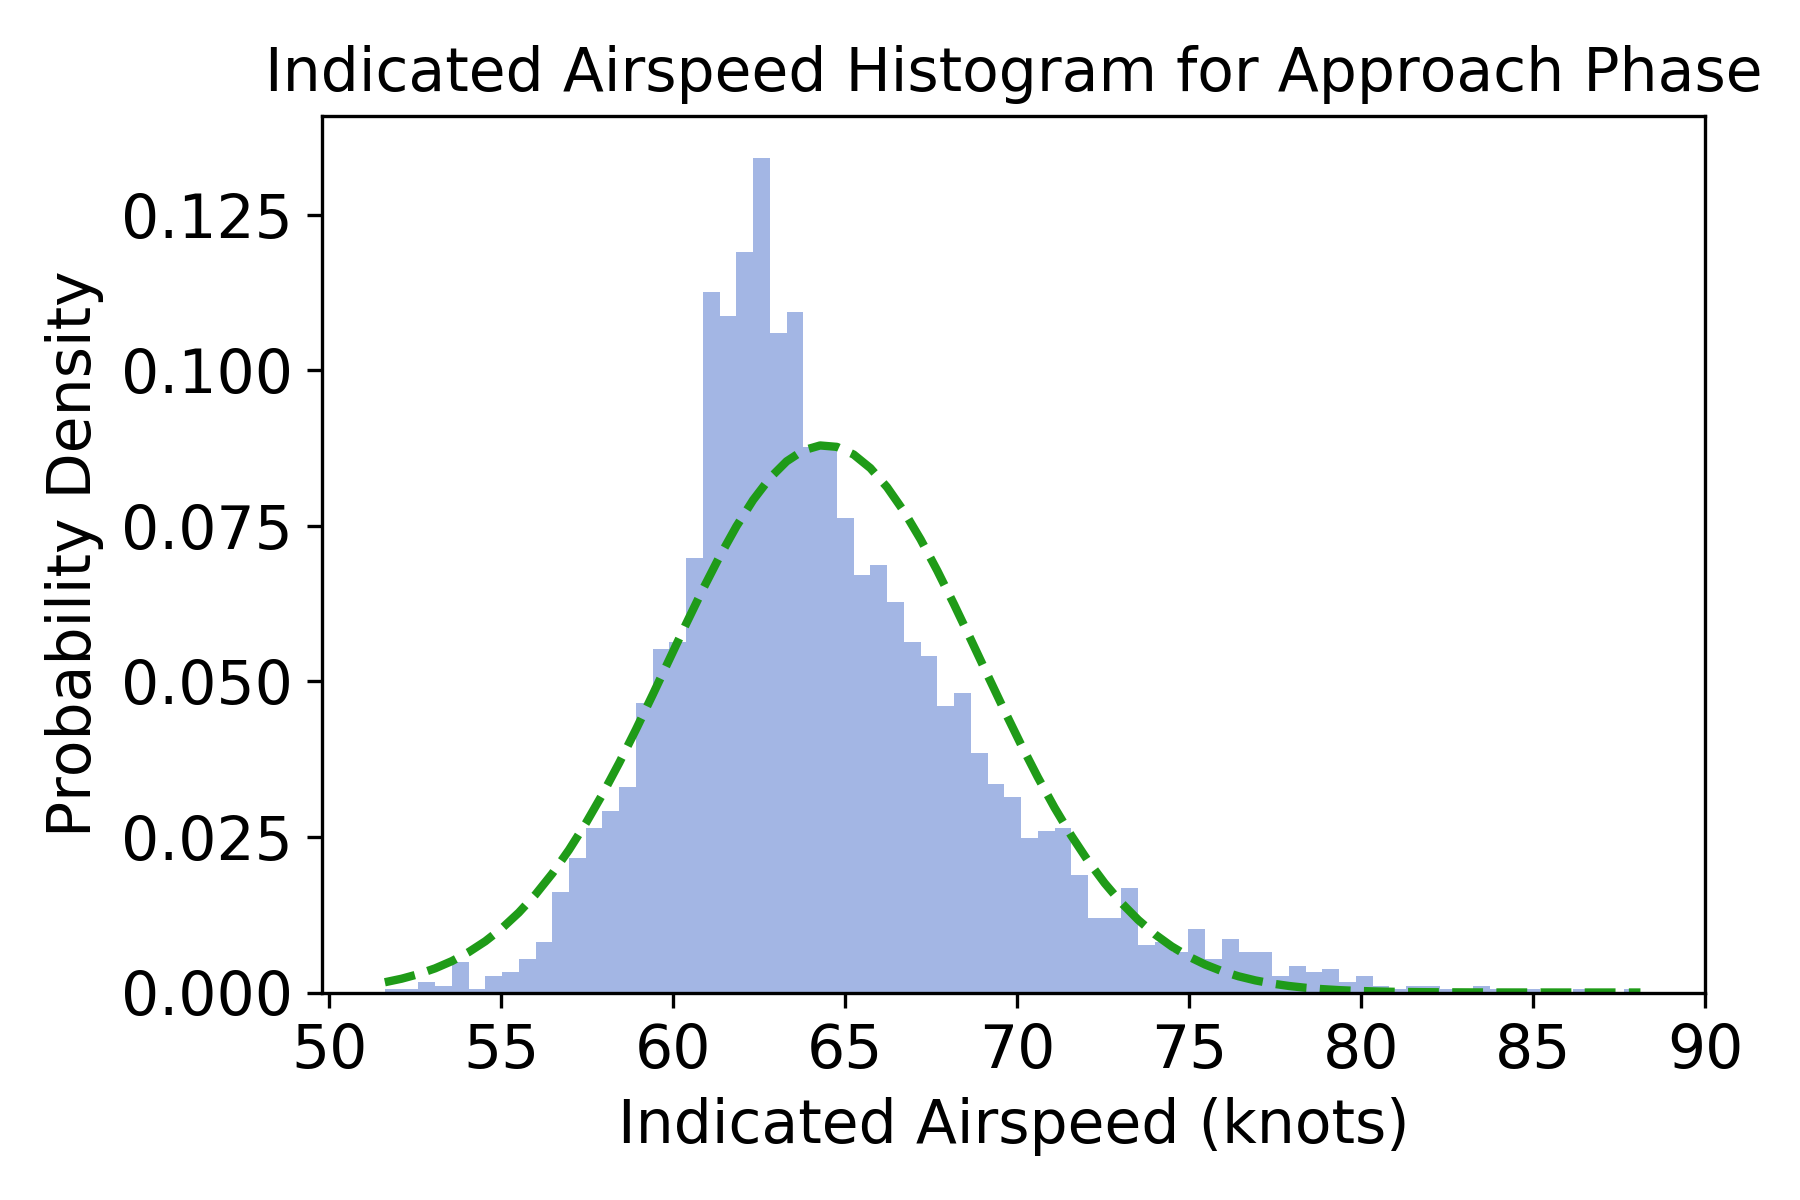
\includegraphics[width=0.45\linewidth]{orig_ias_hist}
        }\hfill%
        \subfloat[Vertical speed indicated.\label{subfig:approach_vsi_hist}]{
        	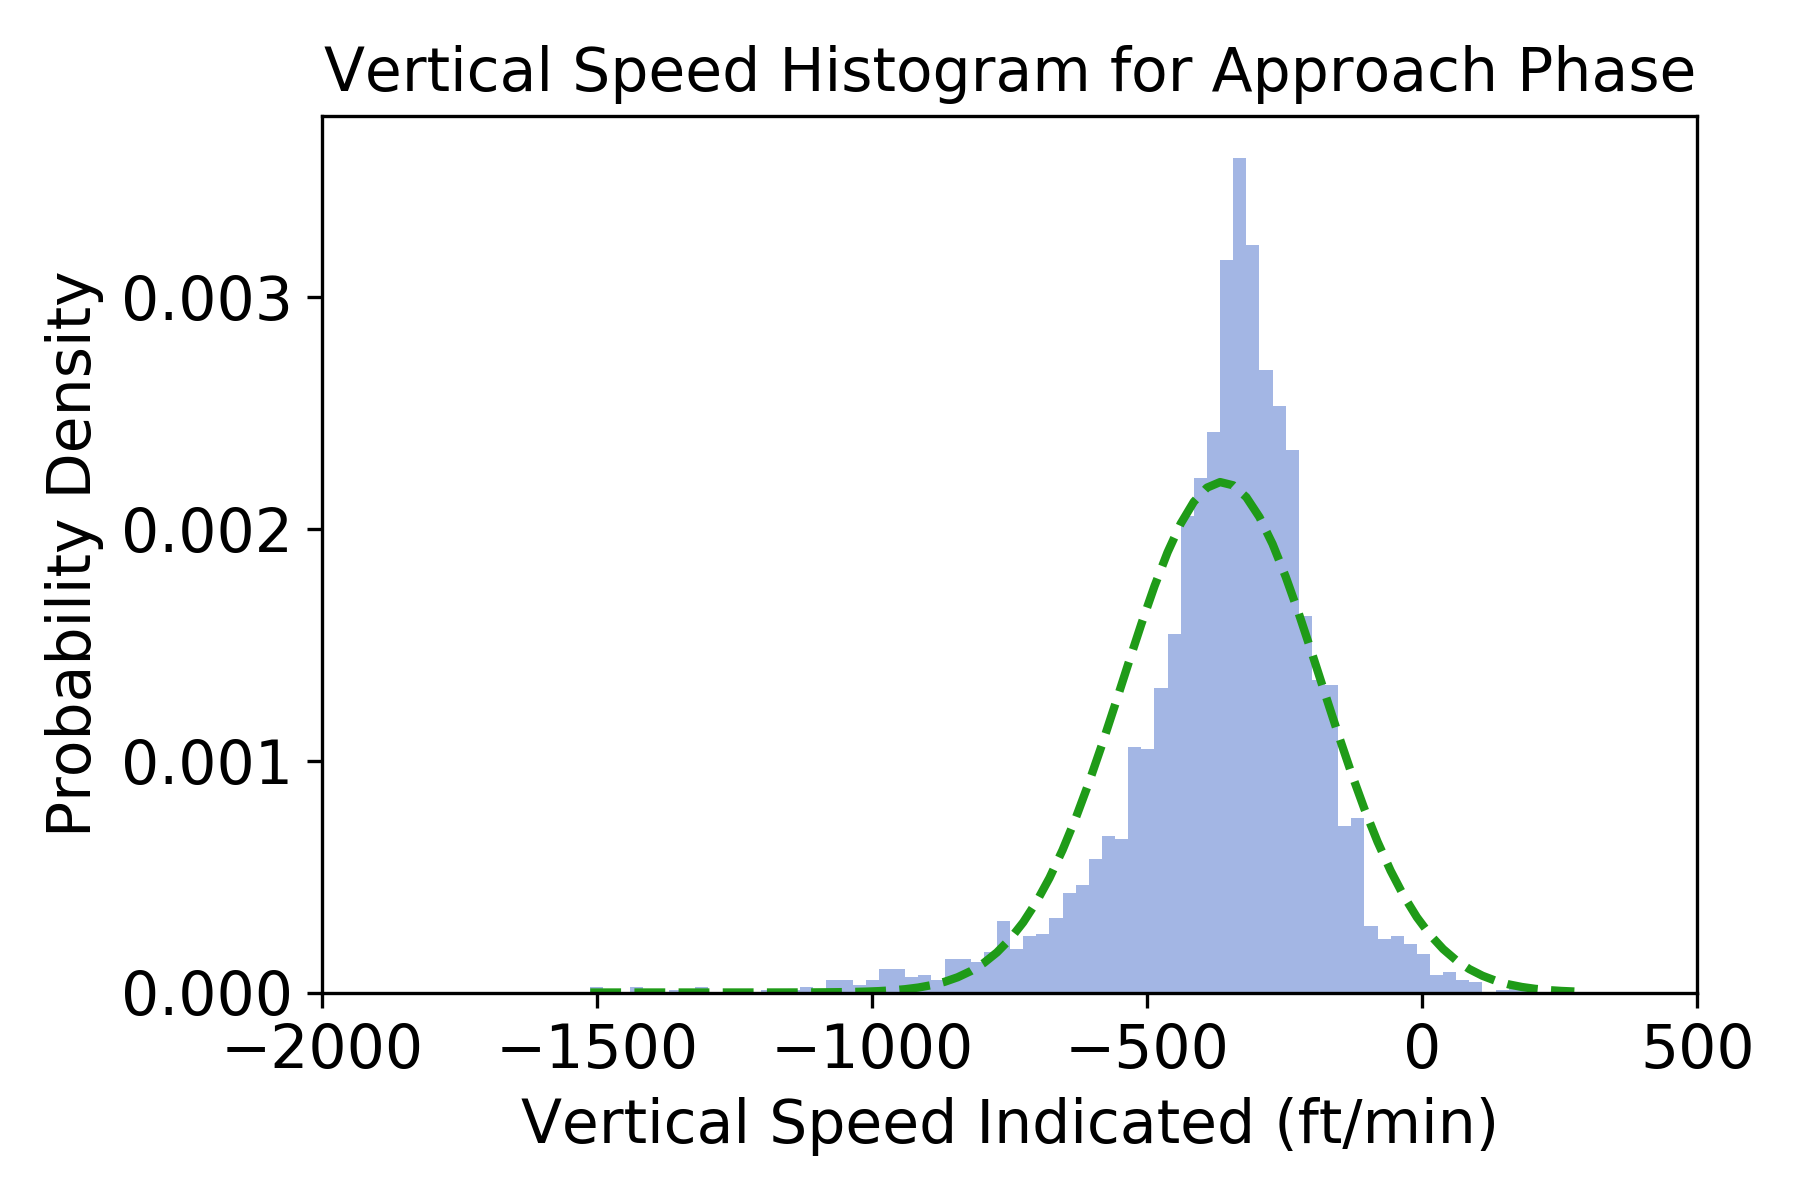
\includegraphics[width=0.45\linewidth]{orig_vsi_hist}
        }%
        
        \subfloat[Cross track error.\label{subfig:approach_cross_track_hist}]{
        	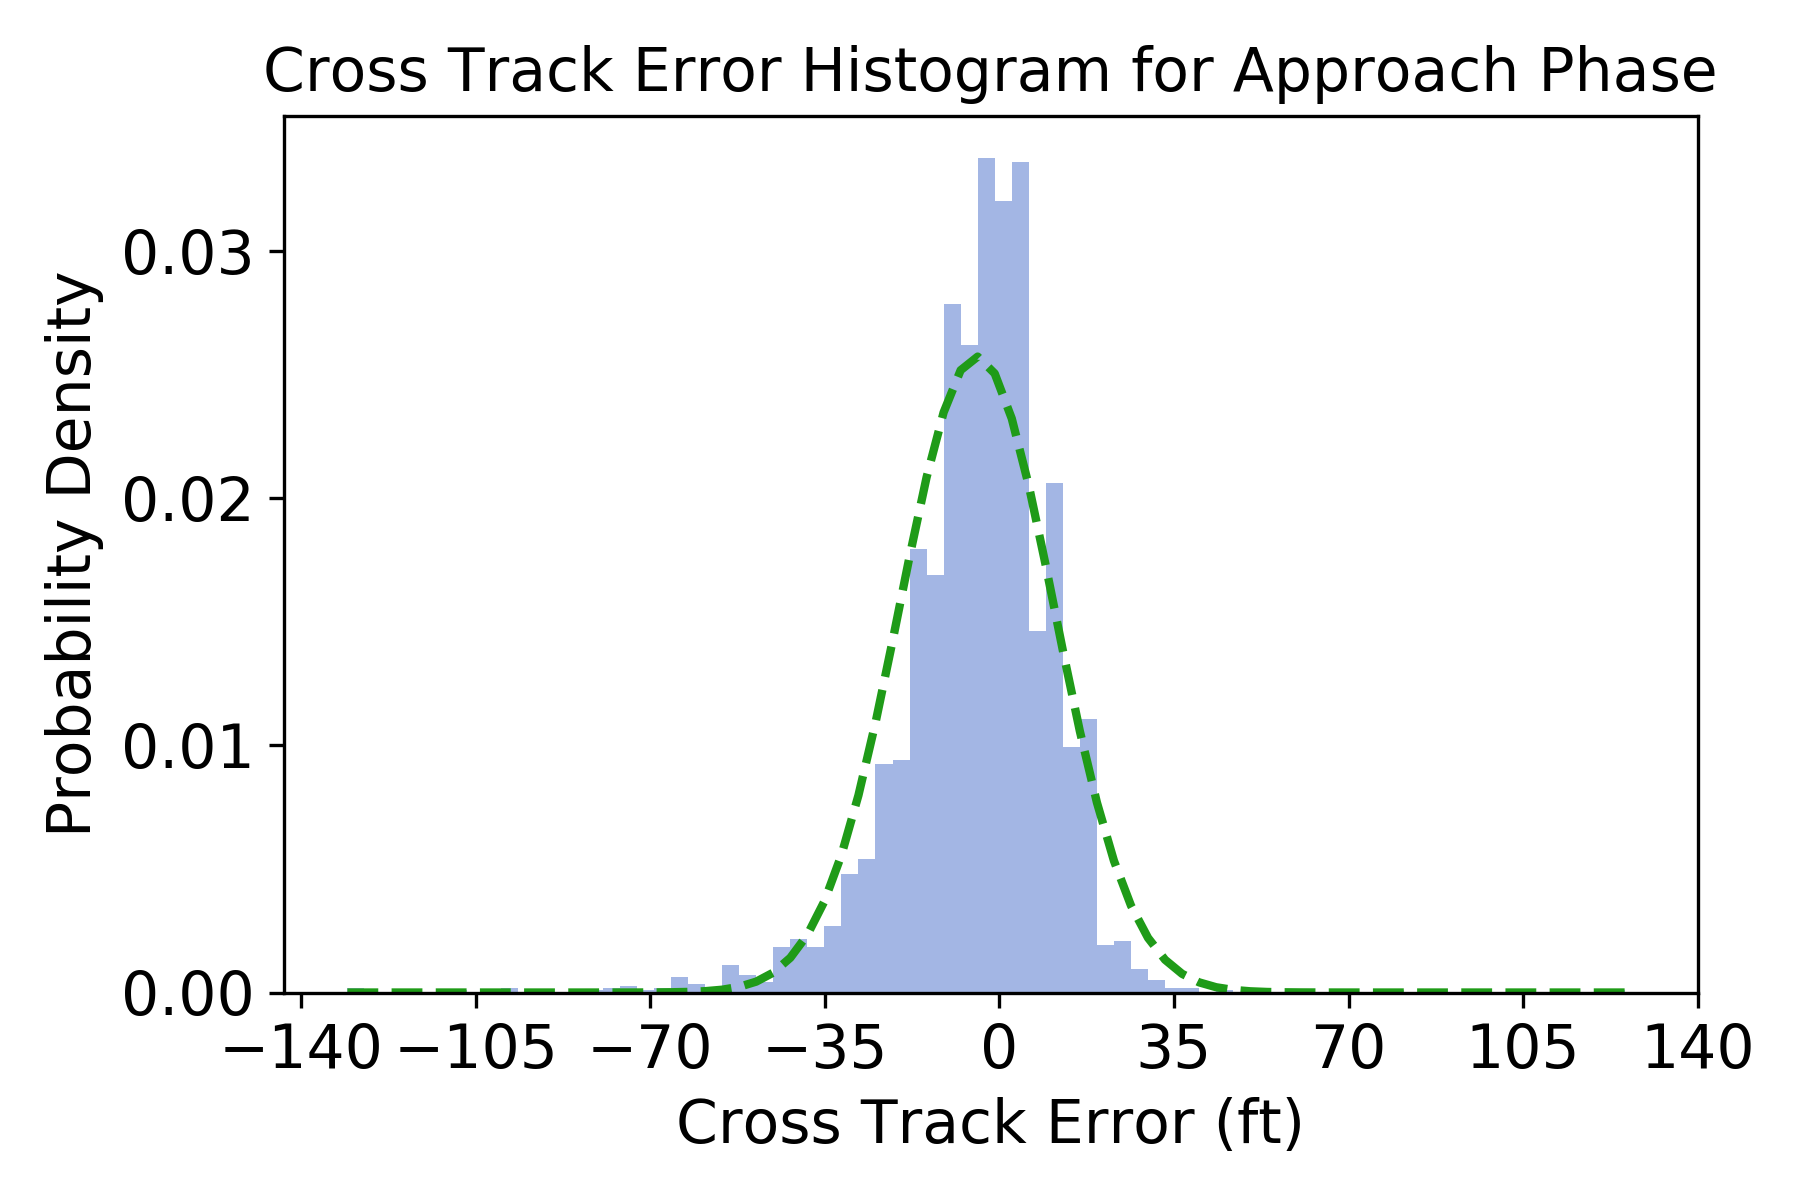
\includegraphics[width=0.45\linewidth]{orig_cross_track_hist}
        }\hfill%
        \subfloat[Heading error.\label{subfig:approach_heading_hist}]{
        	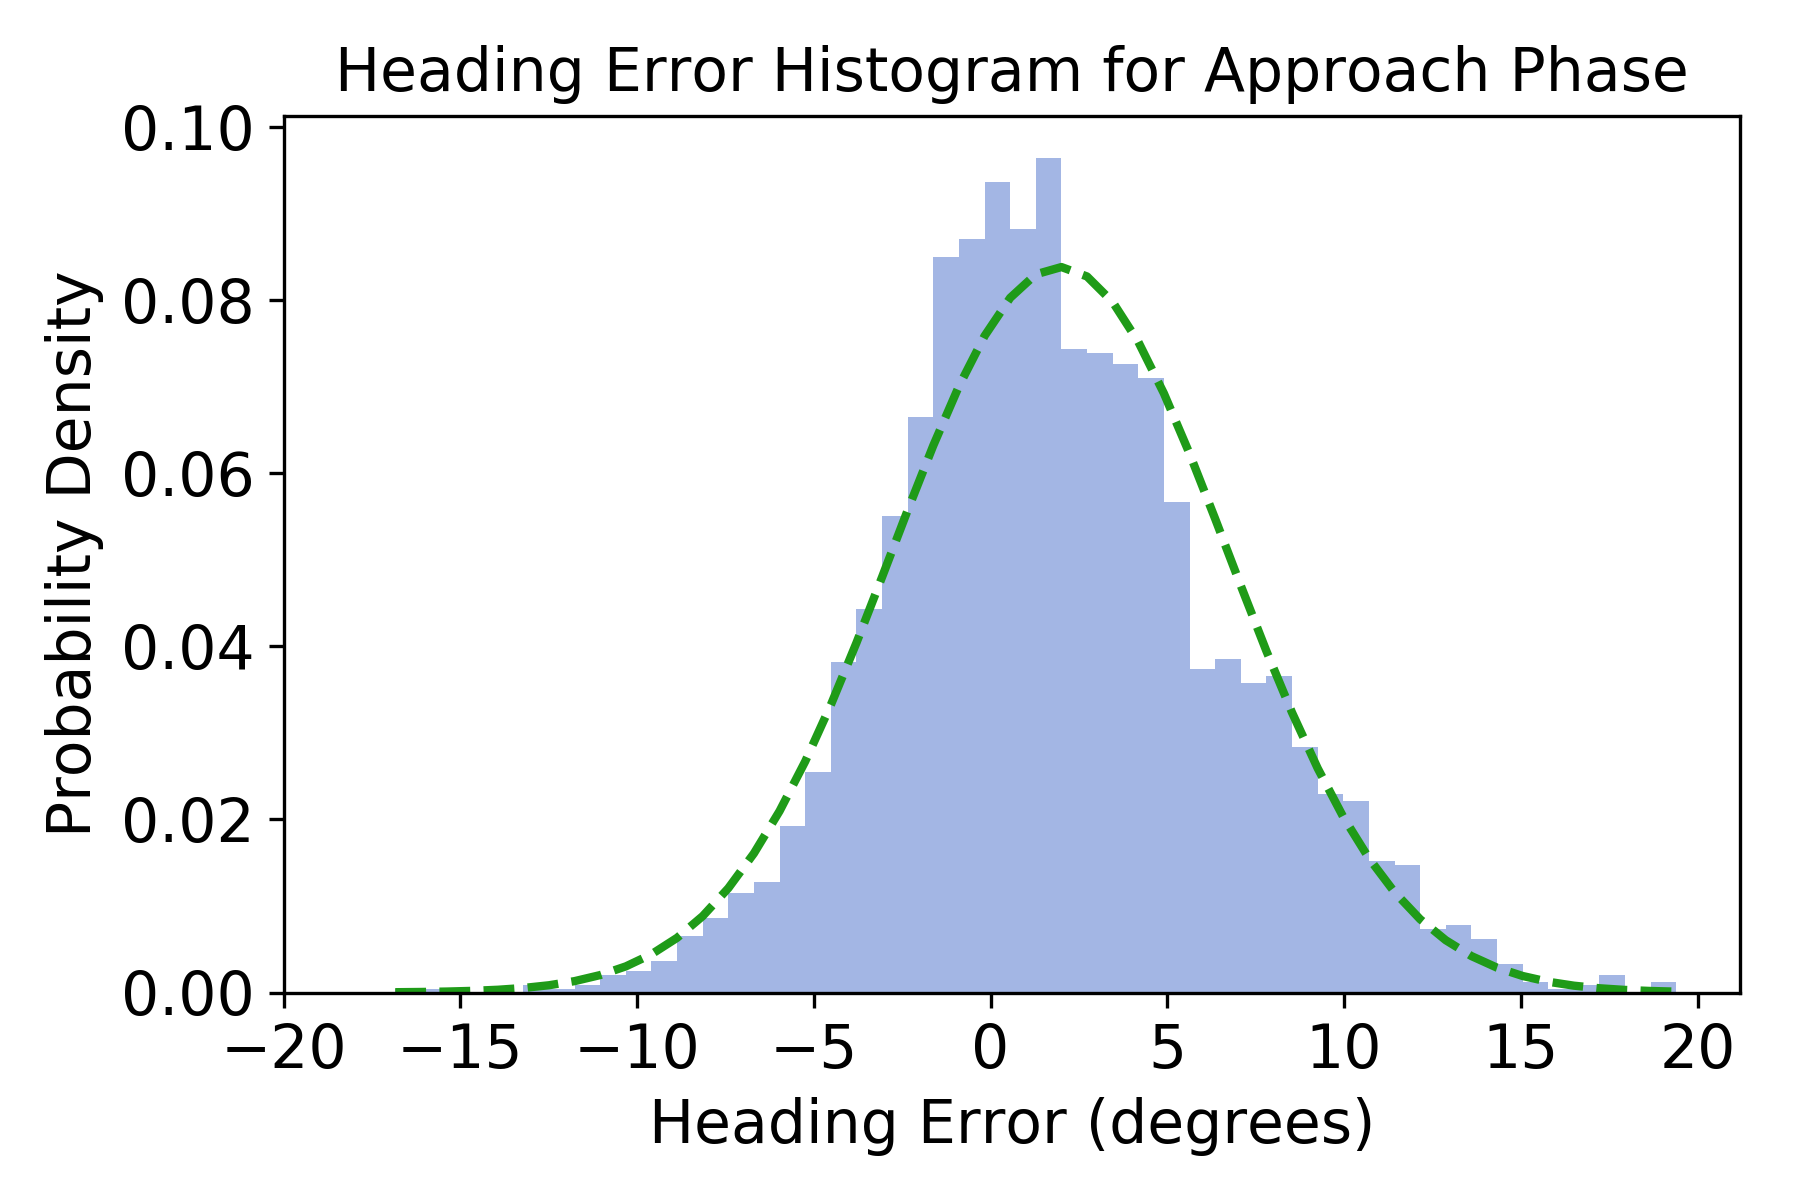
\includegraphics[width=0.45\linewidth]{orig_heading_hist}
        }%
        \caption{Histograms showing the frequencies of values for each parameter during all Approach phases.  Each graph also has a dotted best-fit line to show how close the frequencies adhere to a normal distribution.}
        \label{fig:approach_histograms}
    \end{figure}
    
    
    	%----------
        % FINAL TURN
        %----------
        \subsubsection{Final Turn.}
        
        	Out of the 380 detected approaches; 262 (68.95\%) had a Final Turn subphase, 76 (20.00\%) performed a straight-in approach, and 42 (11.05\%) were not able to detect the runway and, therefore, could not detect whether a Final Turn was performed.  \Cref{fig:final_turn_results_ratios} depicts these ratios.  As mentioned earlier, the 42 \textit{null} runways will be drastically reduced in the future once additional airports and runways are added to the geological database.  Once the airport and runway databases are more complete, the runway error rate should become much more acceptable.
            
            \Cref{fig:final_turn_results_by_risk} gives a comparison of the number of occurrences for each turn error type and Risk Level classification.  This graph is displaying the subset of 262 detected Final Turn subphases found in \Cref{fig:final_turn_results_ratios}.  The figure shows that 76.34\% of the Final Turns resulted in an undershoot and a large proportion (45.420\%) resulted in a Risk Level 2 undershoot.  Those statistics are definitely interesting and are an example of an anomaly that is worth looking into by an aviation expert.  One explanation could be that there is frequently a strong wind component against the aircraft, which could cause the numerous undershoots.  Further analysis such as this could be performed as a future work since wind and other meteorological factors were not taken into consideration in the analyses within this research.
            
            \begin{figure}
            	\centering
                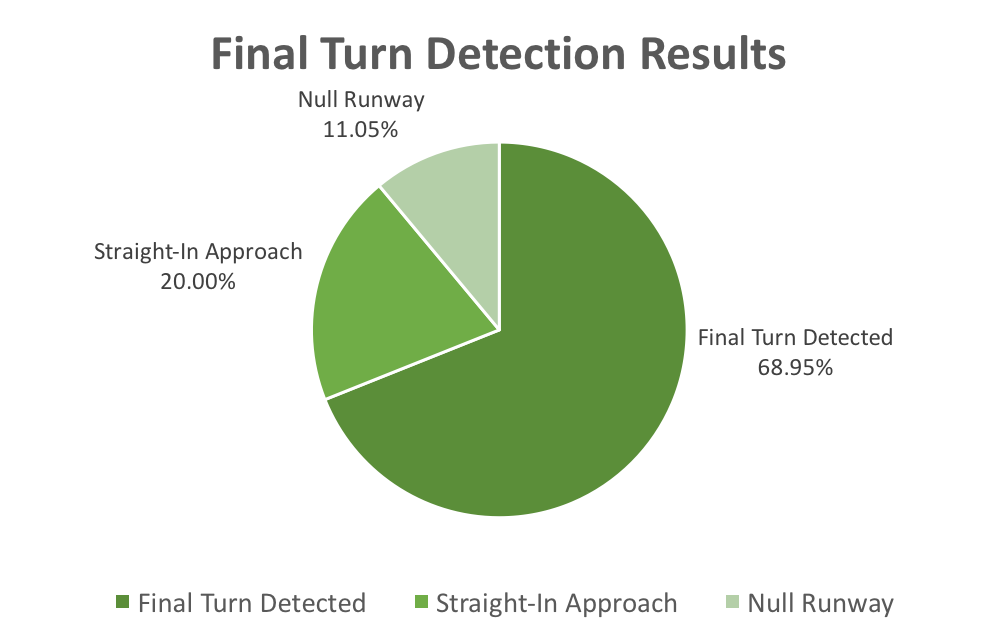
\includegraphics[width=0.75\linewidth]{final_turn_detection_results}
                \caption{Pie chart showing the results from the Final Turn detection algorithm.}
                \label{fig:final_turn_results_ratios}
            \end{figure}
            
            \begin{figure}
            	\centering
                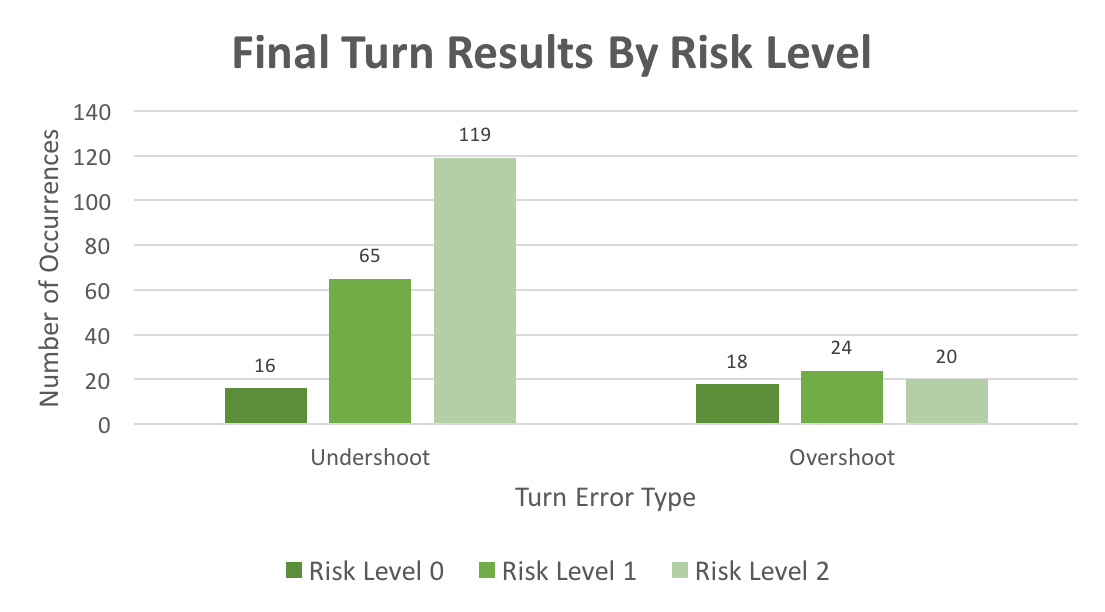
\includegraphics[width=0.95\linewidth]{final_turn_results_by_risk}
                \caption{Frequency of the occurrences of each turn error type for Risk Levels 0, 1, and 2.}
                \label{fig:final_turn_results_by_risk}
            \end{figure}
            
        
        %----------
        % SELF-DEFINED GLIDE PATH
        %----------
%         \subsubsection{Self-defined glide path.}
        
%         	\note{Not sure.  May remove this section since the Web Interface shows exactly the charts that can be created.}


%----------------------------------------
% GRADING METRICS: DEFINE FROM PARAMETER FREQUENCIES
%----------------------------------------
\section{Grading Metrics:  Define From Parameter Frequencies}

	As mentioned in \Cref{ch:methodology}, the goal for creating the Risk Level metrics is to use statistical results from the Approach quality analysis to determine reasonable values that still adhere to the published stable value ranges.  \Cref{subfig:approach_ias_hist,subfig:approach_vsi_hist,subfig:approach_cross_track_hist,subfig:approach_heading_hist} above contain normalized histograms showing the probability density for the parameter values.  These graphs were analyzed by an aviation statistics expert from UND in order to create a safe range (Risk Level 0), a moderate risk range (Risk Level 1), and a high risk range (Risk Level 2) for each parameter of concern.  These graphs will be re-used in the following Sections, but will have additional information showing the value ranges that were created.  The Risk Level 1 values will be a yellow dotted line, while the Risk Level 2 values will be a red dotted line.  A summary of the defined grading metrics can be seen in \Cref{tab:metrics_values} at the end of this Section.
    
    	
    %----------
    % IAS
    %----------
    \subsection{Indicated Airspeed Between 55 and 75 knots}
    
          The indicated airspeed values had a mean of 64.401 knots and a standard deviation of 4.535 knots.  The aviation expert stated that the UND standardization manual~\cite{und_flight_manual} has a strict safe range of 61 -0/+5 knots, and thus anything less than 61 knots should be automatically classified as a Risk Level 2.  He advised the higher Risk Level 1 should begin with any value greater than 66 knots due to the same rule.  Lastly, he advised setting the higher Risk Level 2 at 71 knots in order to use the consistent 5 knots increment, which is also relatively close to one standard deviation.  As is shown in \Cref{fig:revised_ias_hist}, the graph is slightly skewed to the right following the -0/+5 knots rule, which is more lenient towards faster speeds than slower speeds.

		\begin{figure}
			\centering
            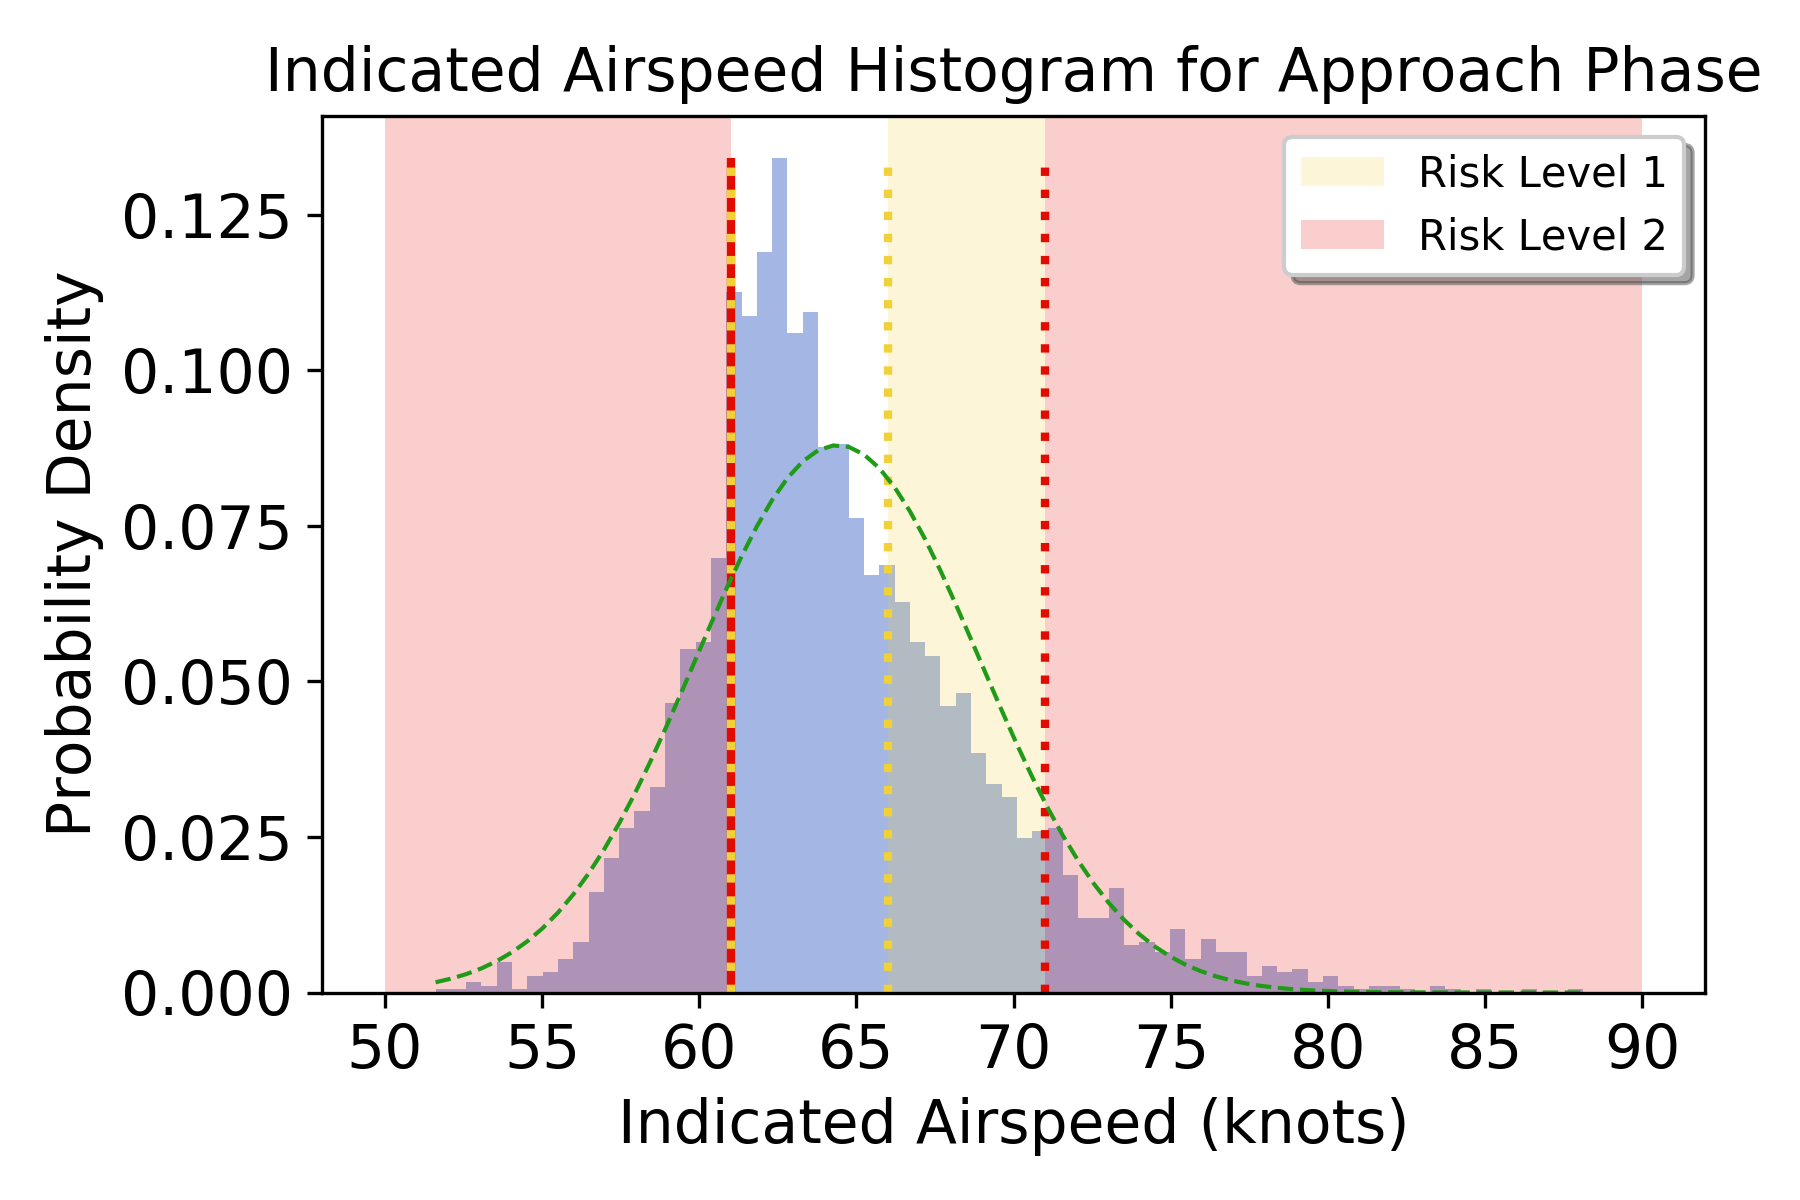
\includegraphics[width=\linewidth]{revised_ias_hist}
            \caption{Histogram for indicated airspeed ($\mu = 64.401, \sigma = 4.535$).  The safe range is between 61 and 66 knots.  There is no lower Risk Level 1 since the Risk Level 2 is anything less than 61 knots.  The higher Risk Level 1 range is between 66 and 71 knots, and the Risk Level 2 is anything greater than 71 knots.}
            \label{fig:revised_ias_hist}
		\end{figure}



    %----------
    % VSI
    %----------
    \subsection{Vertical Speed Indicated Greater Than -1000 ft/min}
    
    	The vertical speed indicated values had a mean of -364.528 ft/min and a standard deviation of 181.210 ft/min.  Although the UND standardization manual states that a vertical speed greater than -1000 ft/min should be achieved for a stabilized approach, the aviation expert stated that a safe range of -800 to -500 ft/min is typically suggested instead of the wide range provided in the manual.  The lower Risk Level 1 is any value that is less than -800 ft/min, and the lower Risk Level 2 is any value less than -1000 ft/min in order to adhere to the stable limit given in the manual.  The higher Risk Level 1 is any value greater than -500 ft/min, and the higher Risk Level 2 is any value greater than -250 ft/min.  These higher limits were chosen because if the aircraft is descending at 250 ft/min, it will typically result in an unsafe and shallow glide slope.  \Cref{fig:revised_vsi_hist} shows these limits and shows that the values are slightly skewed to the left, which corresponds to the risk limits that we've set.

		\begin{figure}[t]
			\centering
            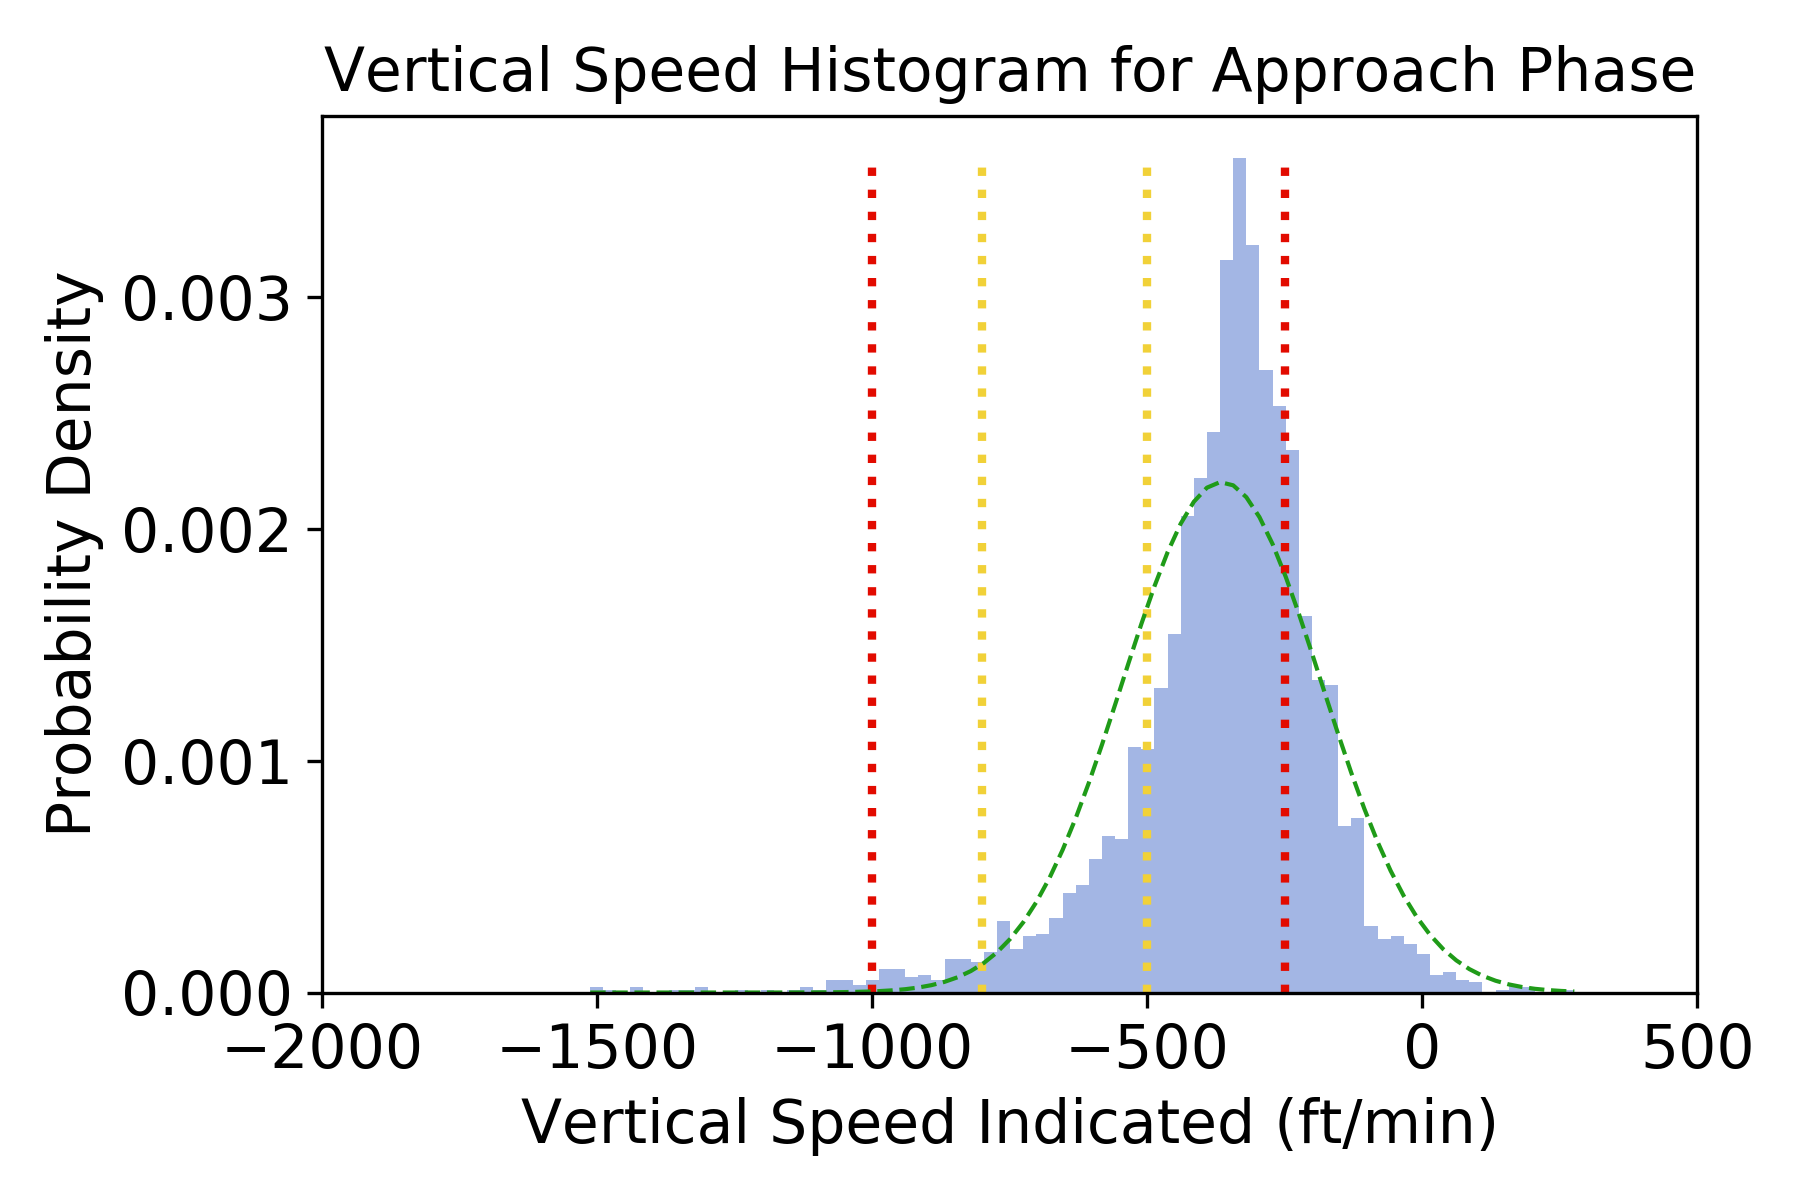
\includegraphics[width=\linewidth]{revised_vsi_hist}
            \caption{Histogram for vertical speed indicated ($\mu = -364.528, \sigma = 181.210$).  The safe range is between -800 and -500 ft/min.  The lower Risk Level 1 range is between -1000 and -800 ft/min, and the Risk Level 2 is anything less than -1000 ft/min.  The higher Risk Level 1 range is between -500 and -250 ft/min, and the Risk Level 2 is anything greater than -250 ft/min.}
            \label{fig:revised_vsi_hist}
		\end{figure}



    %----------
    % CROSS TRACK ERROR
    %----------
    \subsection{Absolute Cross Track Error Less Than 50 ft}
    
    	The cross track error values had a mean of -4.542 feet and a standard deviation of 15.499 feet.  \Cref{fig:revised_cross_track_hist} displays the histogram for these values and it can be seen that the graph is relatively normal with a slight skew to the left.  The aviation expert stated that a deviation in cross track error is not as risky as a deviation in airspeed or vertical speed.  Thus, a wider safe range was defined as -40 feet to 40 feet, which is about where the tails wane on both sides.  Consequently, the lower and higher Risk Level 1 ranges are -50 feet to -40 feet and 40 feet to 50 feet, respectively.  The lower and higher Risk Level 2 values are then -50 feet and 50 feet, respectively, in order to correspond with the original stable limits that were used.
        
		\begin{figure}[t]
			\centering
            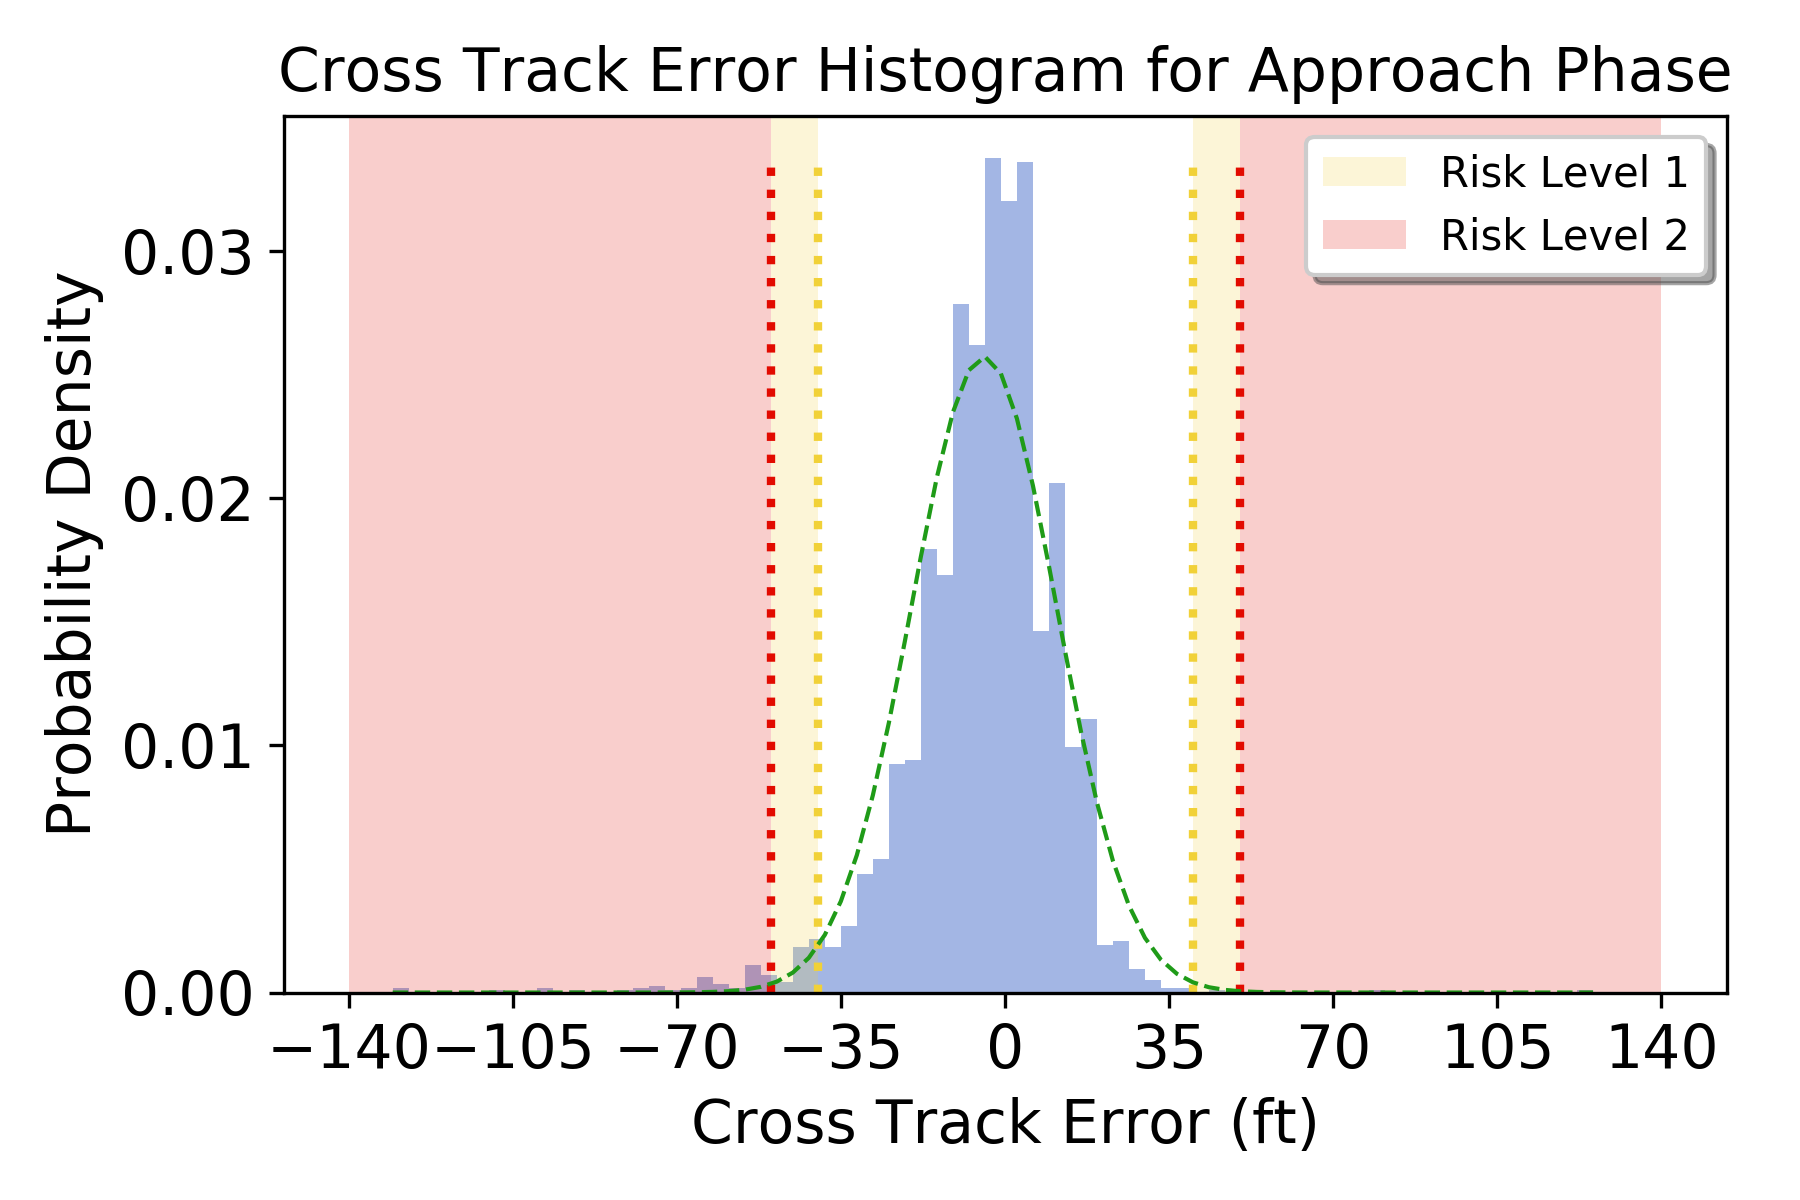
\includegraphics[width=\linewidth]{revised_cross_track_hist}
            \caption{Histogram for cross track error ($\mu = -4.542, \sigma = 15.499$).  The safe range is between -40 and 40 ft.  The lower Risk Level 1 range is between -50 and -40 ft, and the Risk Level 2 is anything less than -50 ft.  The higher Risk Level 1 range is between 40 and 50 ft, and the Risk Level 2 is anything greater than 50 ft.}
            \label{fig:revised_cross_track_hist}
		\end{figure}



    %----------
    % HEADING ERROR
    %----------
    \subsection{Absolute Heading Error Less Than 10 degrees}
    
    	The heading error values had a mean of $1.958^\circ$ and a standard deviation of $4.761^\circ$.  Similar to cross track error, the aviation expert stated that heading error is not as risky as error in the other parameters.  He also mentioned that heading error is slightly more difficult to judge without knowing the wind component on the aircraft since the pilot may have to purposely direct the aircraft several degrees off-center in order to counteract the push of the wind.  Both of these facts means that the safe range for heading error will contain a majority of values.  With that said, the expert advised using a safe range of $-15^\circ$ to $15^\circ$.  The lower and higher Risk Level 1 ranges are from $-20^\circ$ to $-15^\circ$ and $15^\circ$ to $20^\circ$, respectively.  Consequently, the lower and higher Risk Level 2 values are $-20^\circ$ and $20^\circ$, respectively.  The histogram for heading error, as shown in \Cref{fig:revised_heading_hist}, appears to best fit a normal distribution.
        
        \begin{figure}
			\centering
            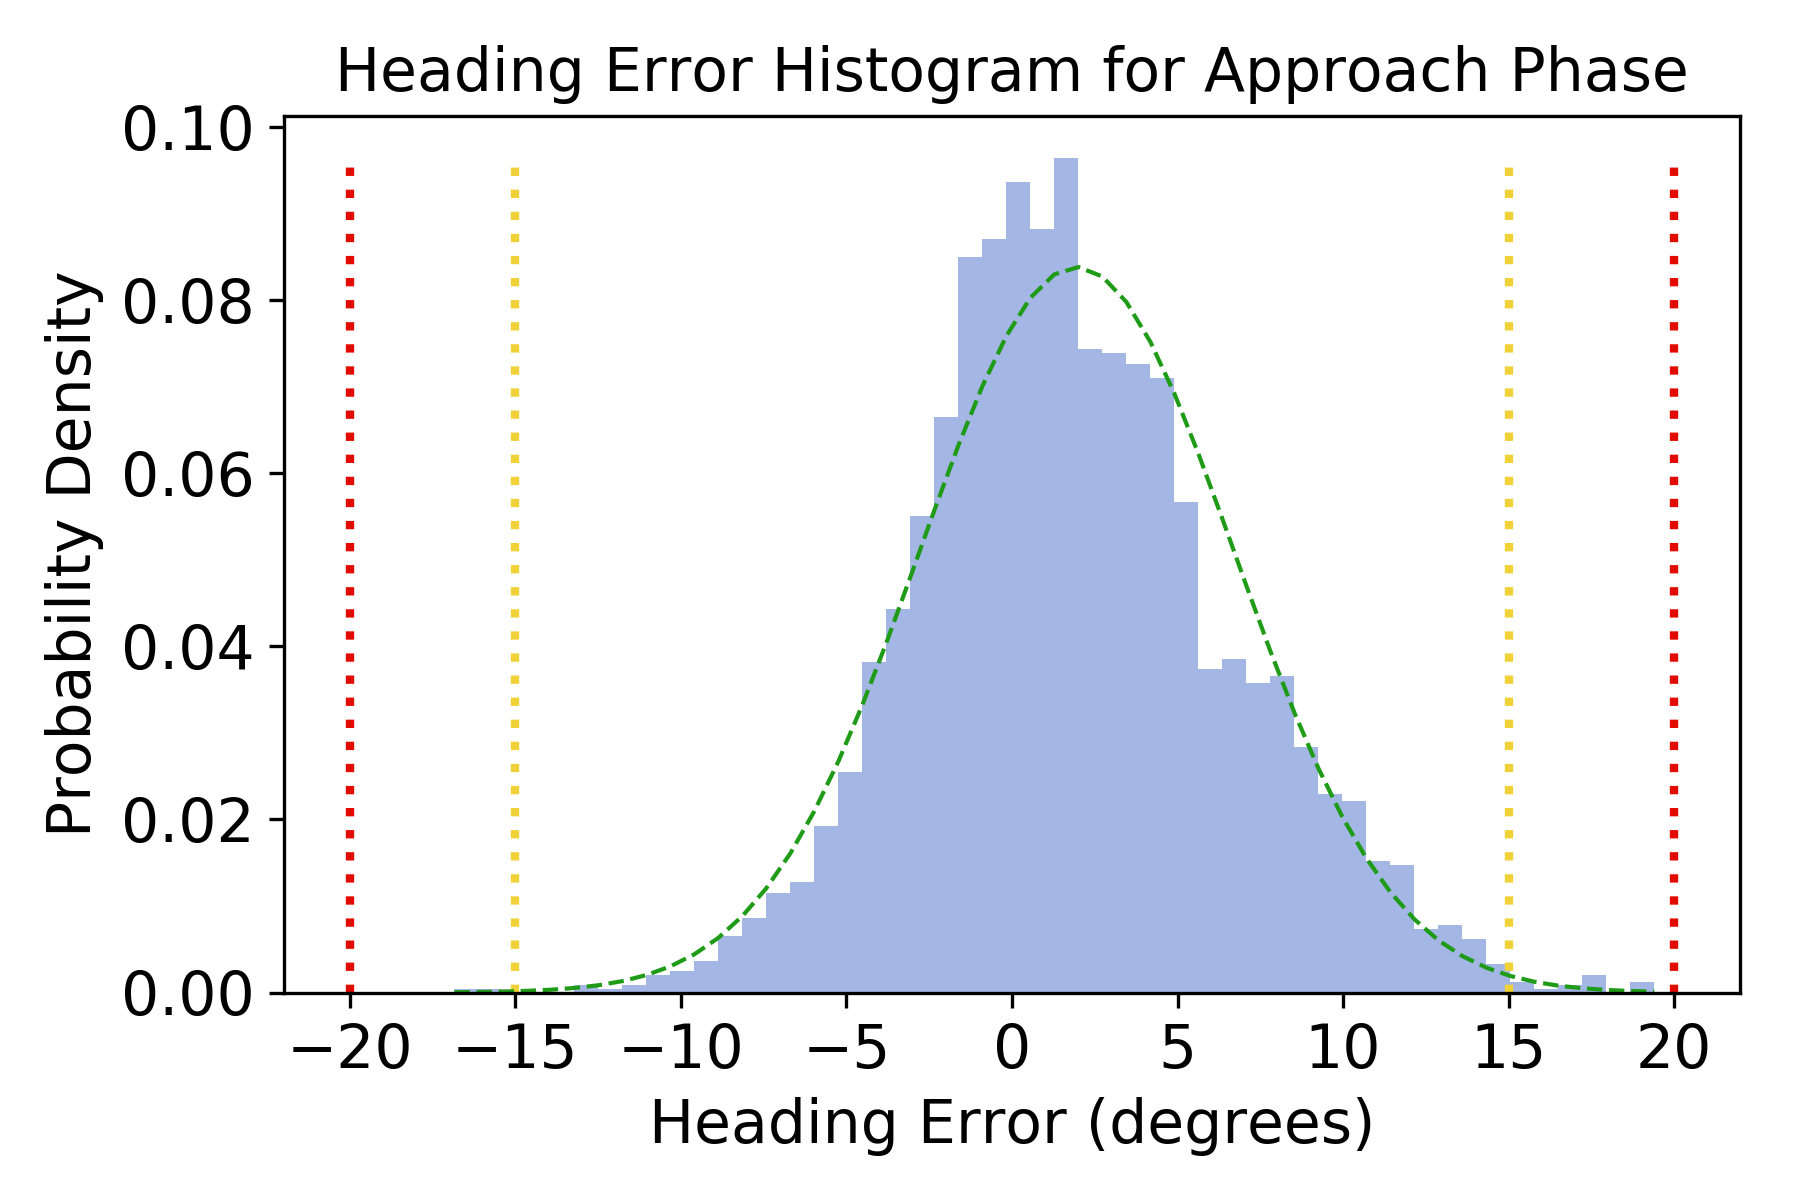
\includegraphics[width=\linewidth]{revised_heading_hist}
            \caption{Histogram for heading error ($\mu = 1.958, \sigma = 4.761$).  The safe range is between -15 and 15 degrees.  The lower Risk Level 1 range is between -20 and -15 degrees, and the Risk Level 2 is anything less than -20 degrees.  The higher Risk Level 1 is between 15 and 20 degrees, and the Risk Level 2 is anything greater than 20 degrees.}
            \label{fig:revised_heading_hist}
		\end{figure}
        
        
        
        \begin{table}
            \centering
            \caption{\small{Defined Risk Levels during Approach for a Cessna C172S}} \label{tab:metrics_values}
            \vspace{3pt}
            \begin{tabular}{@{} l l | r r @{}}
                \hline\noalign{\smallskip}
                \multicolumn{2}{c|}{\bfseries Event} & \bfseries Risk Level 1 & \bfseries Risk Level 2 \\
                \noalign{\smallskip}
                \hline
                \noalign{\smallskip}
                
                \multirow{2}{*}{Indicated Airspeed} & low  & N.A.     & 61 knots \\
                                                    & high & 66 knots & 71 knots \\ 
                			\midrule
                \multirow{2}{*}{Vertical speed} & low  & -800 ft/min & -1000 ft/min \\
                                                & high & -500 ft/min & -250 ft/min \\
                \midrule
                \multirow{2}{*}{Cross track error} & low  & -40 ft & -50 ft \\
                                                   & high & 40 ft  & 50 ft \\
                \midrule
                \multirow{2}{*}{Heading error} & low  & $-15^\circ$ & $-20^\circ$ \\
                                               & high & $15^\circ$  & $20^\circ$ \\
                \midrule
            \end{tabular}
        \end{table}
            

%----------------------------------------
% GRADING METRICS: RESULTS
%----------------------------------------
\section{Grading Metrics:  Experiment Results}
	
	Using the metrics defined in the previous Section, the sample set of flights was re-analyzed in order to determine the risk levels of each parameter for every approach.  This was done by taking all the values for a parameter during the Approach phase, averaging the values, and determining what risk level range the average fell within.  \Cref{fig:metric_parameter_results} shows the frequency of each parameter grouped by risk level as a result of the re-analysis.  From the graph we can see some trends such as the frequency of Risk Level 1 vertical speeds being abnormally higher than the frequency of Risk Level 1.  This may mean that the sample set contained an abnormal number of Approaches with too low or too high rate of descent.  We can also see that Risk Level 0 made up a majority of occurrences for heading and cross track, which follows the fact that these parameters are typically less risky as mentioned in their previous corresponding Subsections.
	
	\begin{figure}
		\centering
		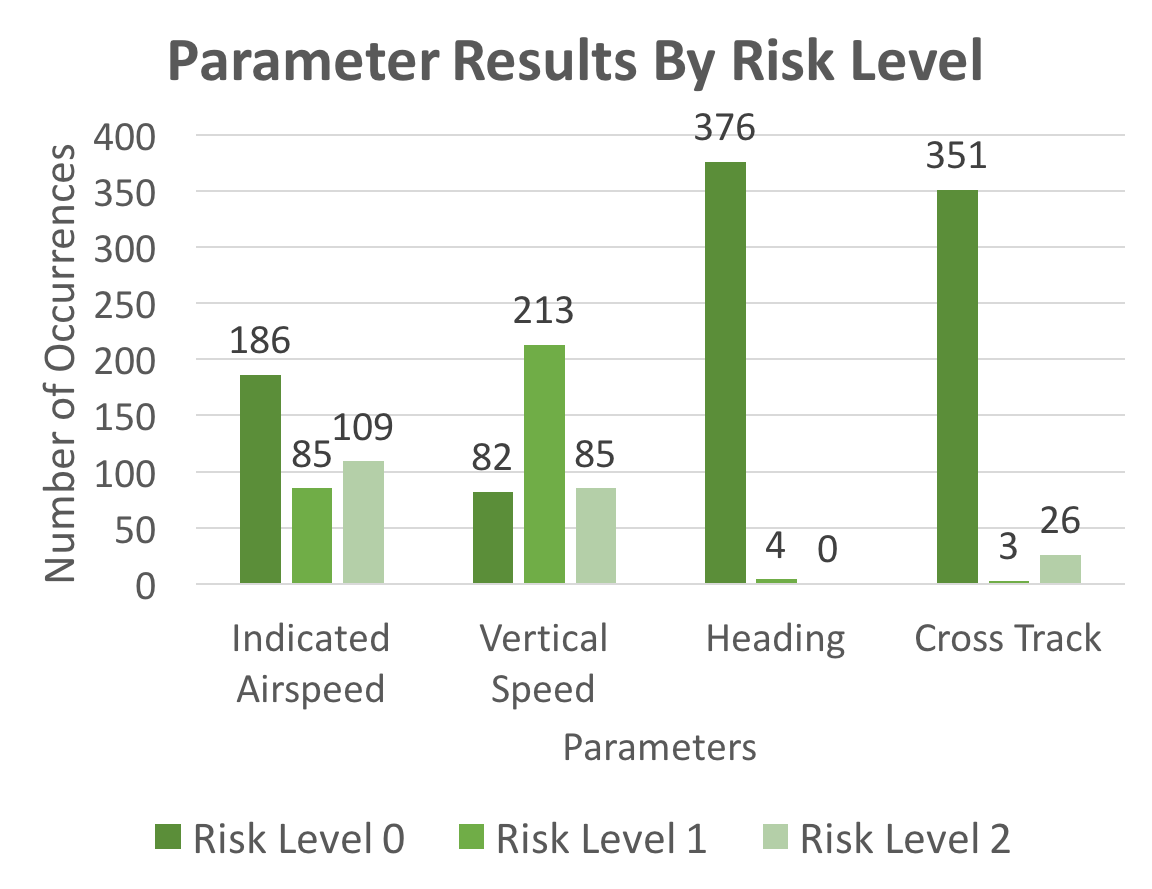
\includegraphics[width=\linewidth]{metric_parameter_results}
		\caption{Frequency of the occurrences of each parameter for Risk Levels 0, 1, and 2 using the newly defined risk level values.}
		\label{fig:metric_parameter_results}
	\end{figure}
	
	
	With regard to grading the Approaches, the total number of deductions is calculated by summing the risk levels across all parameters as well as the Final Turn risk level.  For example; if during an Approach the aircraft achieved a Risk Level 2 in indicated airspeed, a Risk Level 1 in vertical speed, a Risk Level 1 undershoot for the Final Turn, and a Risk Level 0 for all other parameters; the total number of deductions is 4\footnote{$2\,\text{(IAS)} + 1\,\text{(VSI)} + 1\,\text{(Final Turn)} + 0\,\text{(cross track)} + 0\,\text{(heading)} = 4\,\text{deductions}$}.  Additionally, if the aircraft was unstable during the Approach and the pilot did not perform a go-around, an additional one deduction is added to the total.  The total number of deductions is then multiplied by a penalty constant.  The penalty points are subtracted from a total of 100 points in order to obtain the final grade for the Approach.  In this research, a value of 4 points is used as the penalty per deduction.  This value was chosen because there is a possibility of accruing 11 total deductions\footnote{2 risk levels * 4 parameters + 2 Final Turn risk levels + 1 for unstable w/o go-around = 11}, which would create a total of 44 penalty points.  Thus, the worst possible grade to receive would be 56 points\footnote{If using a 90-80-70-60\% grading scale, this would then correspond to an F.}.  \Cref{fig:scores_hist} gives a histogram of the grades calculated for the sample set of 100 flights used during the experiments.  For the grades of the sample set, the mean was 87.168 points and a standard deviation of 7.260 points.  As the figure shows, the histogram reasonably fits a normal distribution, but slightly skewed to the right.  These results have given us good confidence that the grading system will replicate the grading structure already used in Universities that students are already accustomed to.
	
	\begin{figure}
		\centering
		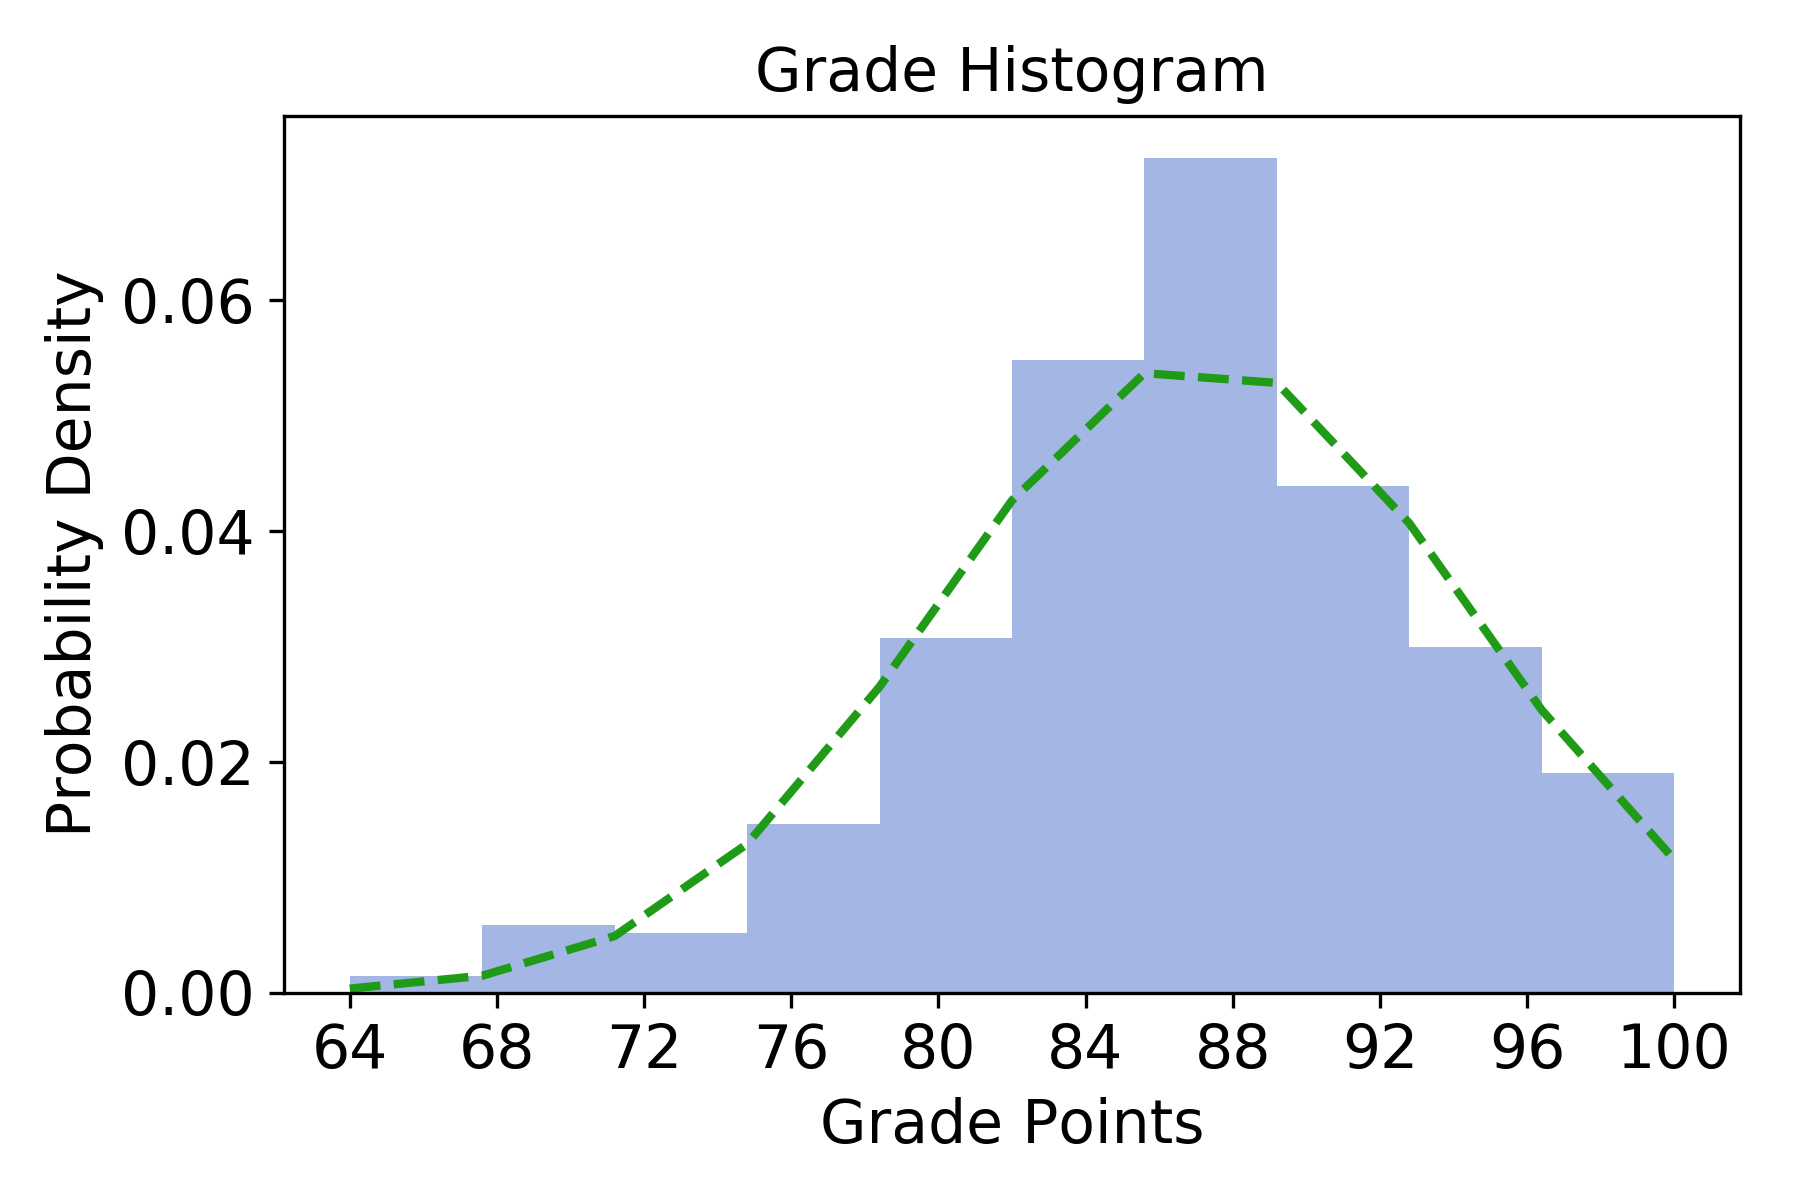
\includegraphics[width=\linewidth]{orig_scores_hist}
		\caption{Histogram showing the results of grading Approach phases.  Each grade is calculated by totaling the risk levels across all parameters then multiplying the sum by a penalty amount per deduction.}
		\label{fig:scores_hist}
	\end{figure}
    
    
%----------------------------------------
% WEB INTERFACES
%----------------------------------------
\section{Web Interfaces}

	This Section details the newly developed web pages for the NGAFID, which dynamically display results based on the user's chosen filters.  At the time of this writing, there have been new tools developed for the Approach, Final Turn, and self-defined glide path analyses.  Each tool will be discussed further in the subsequent Subsections.
    
    
    %----------
    % APPROACH
    %----------
    \subsection{Approach}
    
    	A new web page was implemented in the NGAFID for the purpose of dynamically displaying the Approach analysis results produced by the \toolname\ to users (\Cref{fig:approach_tool_screenshot}).  The results are given in four tabs, one for each parameter, as histograms over a specified date range.  A user is able to dynamically add additional date ranges, which will create an additional series in the chart for comparison.  This feature can be used to detect changes in trends over time.  A user is also, optionally, able to filter the results to an airport and further filter to a single runway.  This will allow users to identify trends that are potentially occurring at a specific runway but not at any other runways.
    
    	\begin{figure}
    		\centering
            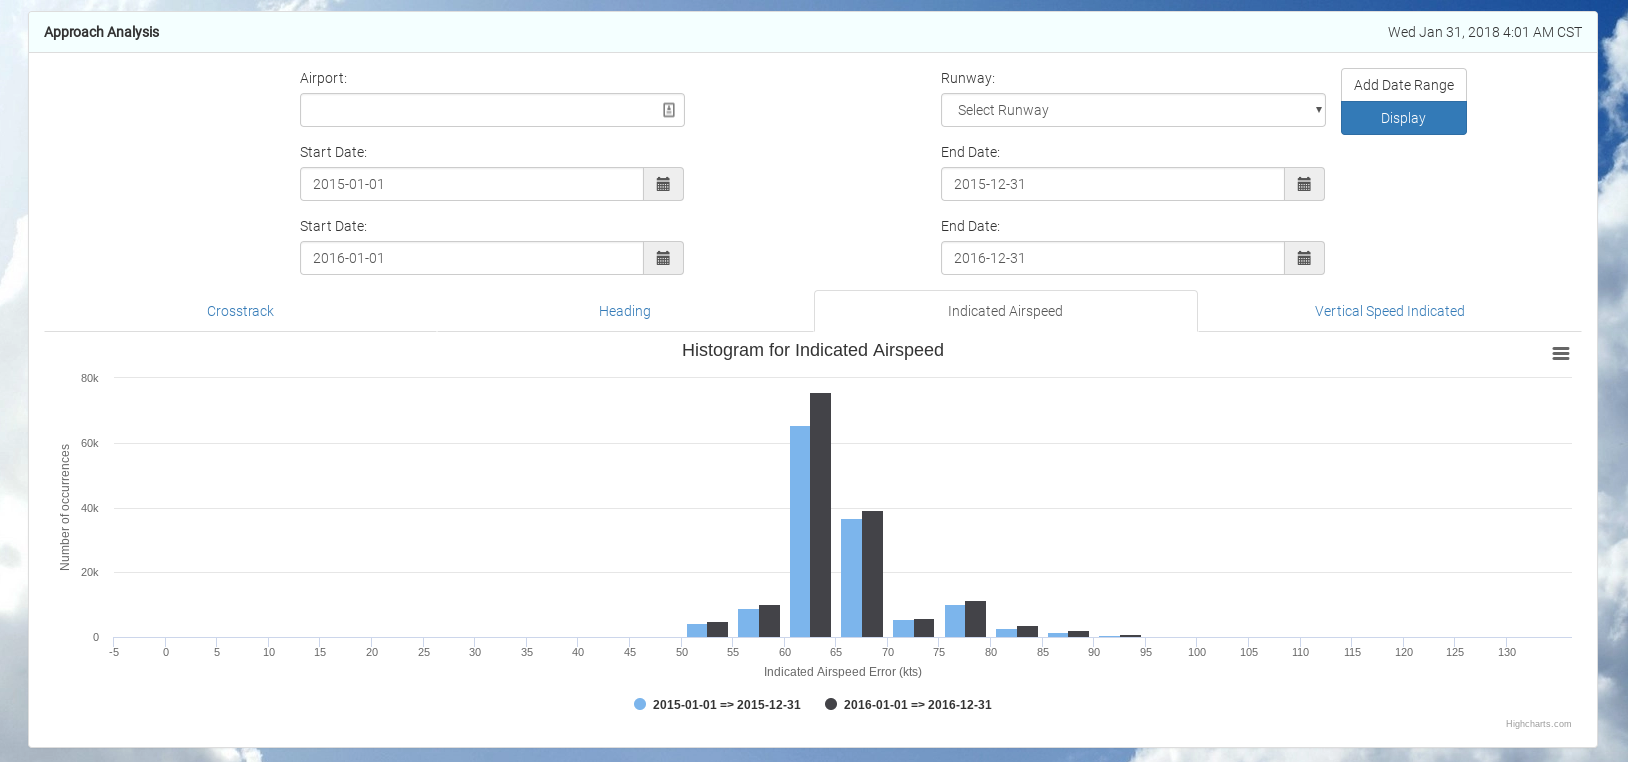
\includegraphics[width=\linewidth]{img/approach_tool_screenshot}
            \caption{A screenshot of the Approach analysis tool on the NGAFID.  It is showing the histogram for indicated airspeed error with two date range filters: 2015-01-01 to 2015-12-31 and 2016-01-01 to 2016-12-31.  The frequency of exceedances can be seen with all values that fall outside of the 55-75 knots range.}
            \label{fig:approach_tool_screenshot}
    	\end{figure}
    
    
    %----------
    % FINAL TURN
    %----------
    \subsection{Final Turn}
    
    	The tool developed for analyzing Final Turn phases in the NGAFID was implemented with two modes:  \textit{(i)} ``Single Flight'' and \textit{(ii)} ``Aggregate''.
    
    	For the ``Single Flight'' mode, the user can input an ID for a specific flight they'd like to analyze (\Cref{fig:single_ttf_screenshot}).  Once the user clicks the ``Display Single Flight'' button, the interactive map then dynamically transitions to the first approach for that flight.  The map will only display one approach at a time; although, there are tabs across the top for each approach which the user can choose.  Once a different tab is chosen, the map automatically transitions the view to that corresponding approach.  The flight path shows different color codings for the separate Final Turn, Approach, and Landing phases as well as different colors for the Final Turn specifically depending on the severity of the turn error.  A Level 1 turn error will be colored yellow, while a Level 2 turn error will be colored red.  If the turn error is less than the Level 1 criteria, it is colored green.  The user is also able to download a PNG screenshot of the map by clicking the ``Download PNG'' button.
        
        For the ``Aggregate'' mode; the user can choose a specific airport, runway, and month and year combination; which will then display all the approaches that occurred at the chosen runway during the chosen time-frame (\Cref{fig:agg_ttf_screenshot}).  This mode allows a user to see trends in Final Turn phases during a given time span.  This mode displays the same color code scheme as the ``Single Flight'' mode.
    
    	\begin{figure}
    		\centering
            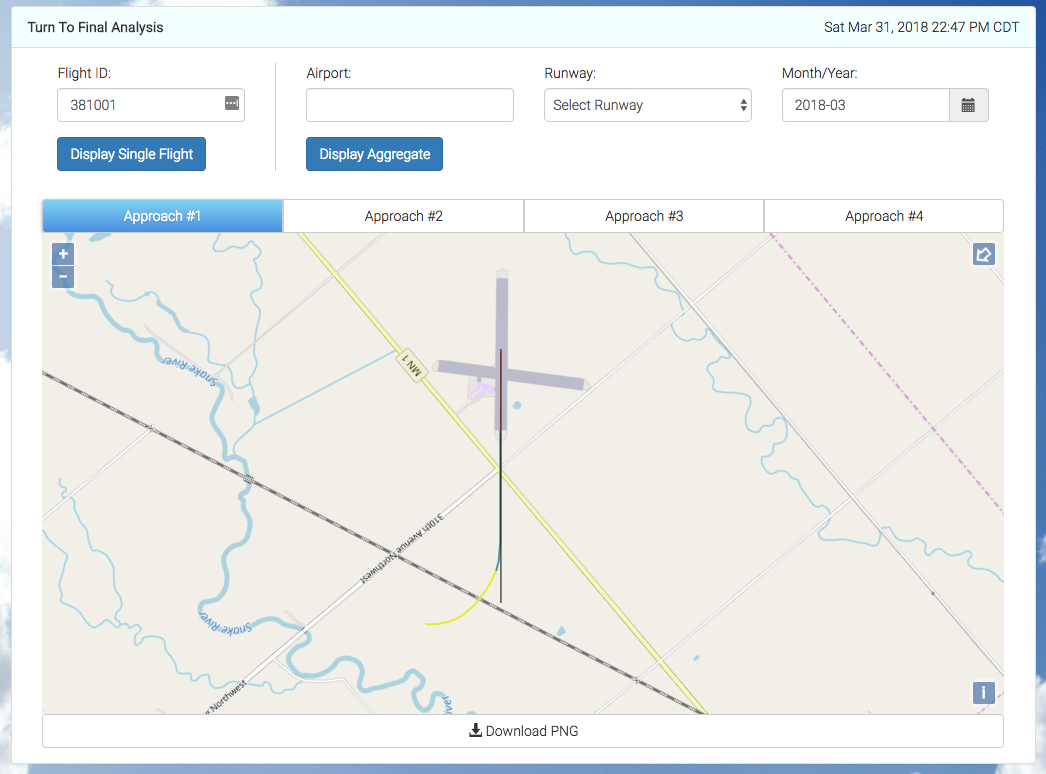
\includegraphics[width=\linewidth]{img/single_ttf_screenshot}
            \caption{A screenshot of the Final Turn analysis tool on the NGAFID in ``Single Flight'' mode.  It is currently showing Approach \#1 for Flight ID \#381001.  Approach \#1 shown here had a Level 1 (yellow color code) undershoot.}
            \label{fig:single_ttf_screenshot}
    	\end{figure}
        
        \begin{figure}
    		\centering
            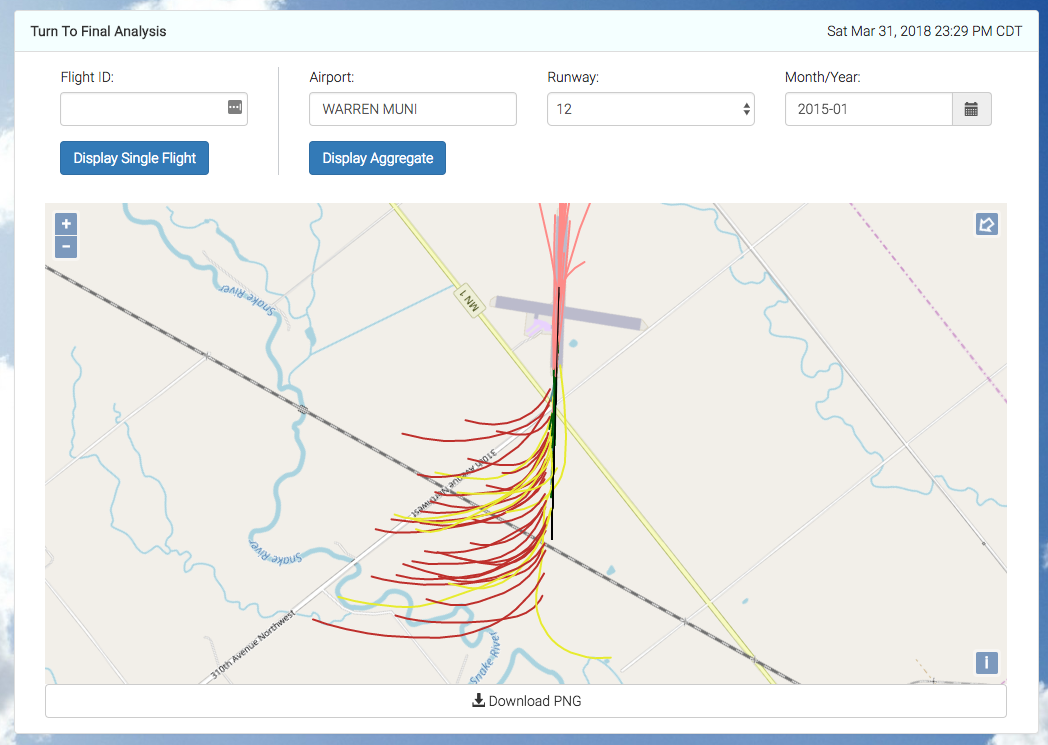
\includegraphics[width=\linewidth]{img/agg_ttf_screenshot}
            \caption{A screenshot of the Final Turn analysis tool on the NGAFID in ``Aggregate'' mode.  It is currently showing all approaches at the Warren Municipal Airport (KD37) for Runway 12 during the month of January 2015.  The many red and yellow lines coming in from the left side mean that a majority of the turns were Level 1 \& 2 undershoots.}
            \label{fig:agg_ttf_screenshot}
    	\end{figure}
    
    %----------
    % SELF-DEFINED
    %----------
    \subsection{Self-Defined Glide Path}
    
    	The tool implemented in the NGAFID for displaying the results of the self-defined glide path analysis currently only supports an aggregate mode (\Cref{fig:self_defined_screenshot}).  It works similarly to the Final Turn tool as the user chooses an airport, runway, and month and year combination.  This will then display a sideways histogram of all the approaches at the given runway during the given time-frame.  The y-axis shows glide path angles from $0^\circ$ to $10^\circ$ in $5^\circ$ increments, and the x-axis shows the number of occurrences that fell within each angle bin.  Lastly, the user can download an image of the displayed chart by clicking the ``hamburger'' menu button.
    
    	\begin{figure}
    		\centering
            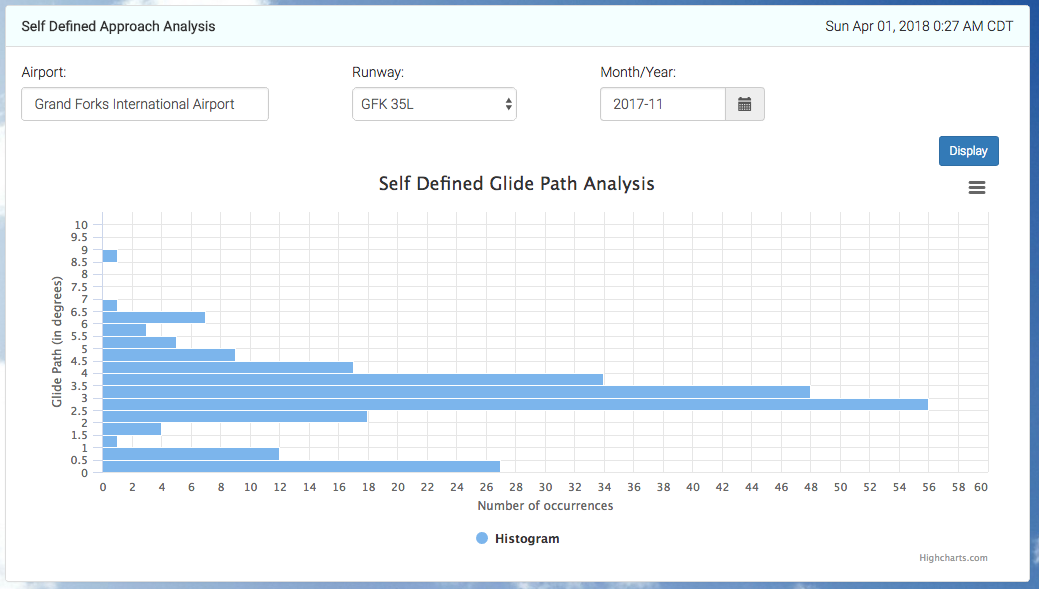
\includegraphics[width=\linewidth]{img/self_defined_screenshot}
            \caption{A screenshot of the Self-Defined Approach analysis tool on the NGAFID.  It is currently showing all approaches at the Grand Forks International Airport (KGFK) for Runway 35L during the month of November 2017.  It displays a sideways histogram with glide path angles on the y-axis and the number of occurrences for each angle on the x-axis.}
            \label{fig:self_defined_screenshot}
    	\end{figure}


%----------------------------------------
% PERFORMANCE
%----------------------------------------
\section{Performance}

	A secondary aspect of this research is to minimize the execution time so the analysis only adds a minimal amount of time to a flight being imported into the NGAFID system.  The results of the benchmarking tests showed that the linearly executing application ran for an average of 127.109 seconds over the 100 randomly tested flights.  On the other hand, the parallel application ran for an average of 56.935 seconds over the same flights.  This means the average per-flight execution times for the linear and parallel applications were 1.271 and 0.569 seconds, respectively.  As a result, the parallelized application had a 2.23x speedup, which is fairly significant.  A summary of the benchmarking tests and other relevant statistics are given in \Cref{tab:performance_results}.
    
    As further evidence, the parallel application was tested on a larger subset of flights to see if the average execution time remained stable, in which it was tested on 5,923 flights.  For this test, the parallel application was able to analyze the data and insert all the results into the database in 2,709.577 seconds.  This gives a per-flight execution time of 0.457 seconds, which is slightly less than the average for 100 flights.  The reasoning behind this can most likely be attributed to the fact that spinning up the sub-processes creates a substantial overhead.  Thus, the longer the application is able to execute, the greater performance gain will be received.  This will, of course, start to show diminishing returns as with any other parallel computing application.
    
    
    \begin{table}[tb]
    	\centering
        \caption{\small{Performance of Linear v. Parallel Execution Times}} \label{tab:performance_results}
        \vspace{3pt}
        \begin{tabular}{@{} >{\centering\arraybackslash} m{.23\linewidth} S[table-format=3.3] S[table-format=2.3] @{}}
            \hline\noalign{\smallskip}
            \bfseries Run \# & \bfseries Linear (sec) & \bfseries Parallel (sec) \\
            \noalign{\smallskip}
            \hline
            \noalign{\smallskip}
             1 & 128.275 & 56.726 \\ \hline
             2 & 130.441 & 56.086 \\ \hline
             3 & 127.878 & 61.263 \\ \hline
             4 & 121.923 & 55.787 \\ \hline
             5 & 126.418 & 57.964 \\ \hline
             6 & 125.425 & 55.753 \\ \hline
             7 & 126.123 & 57.945 \\ \hline
             8 & 128.949 & 55.830 \\ \hline
             9 & 128.161 & 55.497 \\ \hline
            10 & 127.494 & 56.496 \\ \hline
            \hline
            \bfseries Average           & 127.109 & 56.935 \\ \hline
            \bfseries Latency / flight  &   1.271 &  0.569 \\ \hline
            \bfseries Speedup           &         &  2.23x \\ \hline
        \end{tabular}
    \end{table}
    
    
    
    